% Options for packages loaded elsewhere
\PassOptionsToPackage{unicode}{hyperref}
\PassOptionsToPackage{hyphens}{url}
%
\documentclass[
]{article}
\usepackage{lmodern}
\usepackage{amssymb,amsmath}
\usepackage{ifxetex,ifluatex}
\ifnum 0\ifxetex 1\fi\ifluatex 1\fi=0 % if pdftex
  \usepackage[T1]{fontenc}
  \usepackage[utf8]{inputenc}
  \usepackage{textcomp} % provide euro and other symbols
\else % if luatex or xetex
  \usepackage{unicode-math}
  \defaultfontfeatures{Scale=MatchLowercase}
  \defaultfontfeatures[\rmfamily]{Ligatures=TeX,Scale=1}
\fi
% Use upquote if available, for straight quotes in verbatim environments
\IfFileExists{upquote.sty}{\usepackage{upquote}}{}
\IfFileExists{microtype.sty}{% use microtype if available
  \usepackage[]{microtype}
  \UseMicrotypeSet[protrusion]{basicmath} % disable protrusion for tt fonts
}{}
\makeatletter
\@ifundefined{KOMAClassName}{% if non-KOMA class
  \IfFileExists{parskip.sty}{%
    \usepackage{parskip}
  }{% else
    \setlength{\parindent}{0pt}
    \setlength{\parskip}{6pt plus 2pt minus 1pt}}
}{% if KOMA class
  \KOMAoptions{parskip=half}}
\makeatother
\usepackage{xcolor}
\IfFileExists{xurl.sty}{\usepackage{xurl}}{} % add URL line breaks if available
\IfFileExists{bookmark.sty}{\usepackage{bookmark}}{\usepackage{hyperref}}
\hypersetup{
  pdftitle={Installation Guide for the CTT SensorStation and CTT Nodes},
  pdfauthor={support@celltracktech.com},
  hidelinks,
  pdfcreator={LaTeX via pandoc}}
\urlstyle{same} % disable monospaced font for URLs
\usepackage[margin=1in]{geometry}
\usepackage{longtable,booktabs}
% Correct order of tables after \paragraph or \subparagraph
\usepackage{etoolbox}
\makeatletter
\patchcmd\longtable{\par}{\if@noskipsec\mbox{}\fi\par}{}{}
\makeatother
% Allow footnotes in longtable head/foot
\IfFileExists{footnotehyper.sty}{\usepackage{footnotehyper}}{\usepackage{footnote}}
\makesavenoteenv{longtable}
\usepackage{graphicx,grffile}
\makeatletter
\def\maxwidth{\ifdim\Gin@nat@width>\linewidth\linewidth\else\Gin@nat@width\fi}
\def\maxheight{\ifdim\Gin@nat@height>\textheight\textheight\else\Gin@nat@height\fi}
\makeatother
% Scale images if necessary, so that they will not overflow the page
% margins by default, and it is still possible to overwrite the defaults
% using explicit options in \includegraphics[width, height, ...]{}
\setkeys{Gin}{width=\maxwidth,height=\maxheight,keepaspectratio}
% Set default figure placement to htbp
\makeatletter
\def\fps@figure{htbp}
\makeatother
\setlength{\emergencystretch}{3em} % prevent overfull lines
\providecommand{\tightlist}{%
  \setlength{\itemsep}{0pt}\setlength{\parskip}{0pt}}
\setcounter{secnumdepth}{-\maxdimen} % remove section numbering

\title{Installation Guide for the CTT SensorStation and CTT Nodes}
\author{\href{mailto:support@celltracktech.com}{\nolinkurl{support@celltracktech.com}}}
\date{02/10/2021}

\begin{document}
\maketitle

{
\setcounter{tocdepth}{2}
\tableofcontents
}
\begin{center}\rule{0.5\linewidth}{0.5pt}\end{center}

\hypertarget{note-on-version-1-sensorstations-vs.-version-2-sensorstations}{%
\section{Note on Version 1 SensorStations vs.~Version 2
SensorStations}\label{note-on-version-1-sensorstations-vs.-version-2-sensorstations}}

This User Guide has been redesigned around the new (ca.2020) Version 2
SensorStation (V2) which includes an LCD display. Otherwise, Version 1
stations (ca.2019) are nearly identical to V2 stations. In cases where
they differ, we have made note in the manual. If you are setting up a V1
station you may want to begin at the
\protect\hyperlink{V1Quickstart}{QuickStart Guide in Appendix II}. If
you find inconsistencies in this manual please email us at
\href{mailto:support@celltracktech.com}{\nolinkurl{support@celltracktech.com}}
as we will be updating the manual regularly.

\hypertarget{join-us-in-our-slack-user-community}{%
\section{\texorpdfstring{Join us in our \textbf{Slack} User
Community}{Join us in our Slack User Community}}\label{join-us-in-our-slack-user-community}}

We now have a \texttt{Slack} workspace dedicated to CTT users. Topics
range from station logistics to study design, and from data management
to current development of novel analytic tool. Come be a part of the
discussion and engage with other users as we push the boundaries of
remotely sensed telemetry data!
\url{https://join.slack.com/t/celltracktechsupport/shared_invite/zt-m6phfypu-aIV4zznt0Xe3G3oUsC6KRQ}

\hypertarget{congratulations}{%
\section{Congratulations}\label{congratulations}}

If you are reading this document, then you most likely have purchased
one of our Internet of Wildlife (IoW) components. Whether you're doing
localized detailed studies of small mammals or songbirds, or you're
setting up SensorStations as part of the global Motus Wildlife Tracking
System (motus.org), or you're doing something in-between, we've got you
covered, and this document is meant to help you get started quickly and
painlessly. If for some reason you get stuck along the way, please don't
hesitate to reach out to us directly either via email
(\href{mailto:support@celltracktech.com}{\nolinkurl{support@celltracktech.com}})
or through our online Help Desk here:
\url{https://celltracktech.atlassian.net/servicedesk/customer/portals}.

\hypertarget{participating-in-the-motus-wildlife-tracking-system}{%
\section{Participating in the Motus Wildlife Tracking
System}\label{participating-in-the-motus-wildlife-tracking-system}}

If you are setting up your SensorStation to participate in the Motus
Wildlife Tracking System (motus.org), your station can still be used
with CTT Nodes. In general, we recommend Motus stations to include 4
Yagi 10-element antennas pointing in the 4 cardinal directions. A fifth
Omni antenna can be installed and dedicated to detecting nodes, or one
of the Yagi antennas can be used for nodes while the other three are
positioned at 120 degrees for full coverage. You may also add any number
of 166MHz antennas by using a Software Defined Radio (SDR), such as a
FunCube or RTL-SDR, via any of the USB ports on the SensorStation (SDRs
are sold separately via third-party companies). A clear view of the
horizon is preferred to get maximum range, so a height as high as
possible is also advised. For more information on Motus, see
\protect\hyperlink{appendix_1}{Appendix I}.

\hypertarget{sensorstation-precautions}{%
\section{SensorStation Precautions}\label{sensorstation-precautions}}

Treat your SensorStation board like you would any other motherboard,
Arduino or Raspberry Pi. All electronics, no matter how robust, can be
static sensitive. Take care no metal objects touch the board while it is
operating, such as antenna connectors or GSM antennas, as this could
cause electrical shorts that will damage the board. It is advised to
wear an anti-static bracelet when handling SensorStation.


\includegraphics[width=0.25\textwidth,height=\textheight]{/Users/davidlapuma/Dropbox/CTT_Git/ctt_documentation/images/attention.png}

\hypertarget{setting-up-your-ctt-iow-system}{%
\section{Setting up your CTT IoW
System}\label{setting-up-your-ctt-iow-system}}

CTT's Internet of Wildlife System (IoW) is a complete radio telemetry
system that consists of transmitters (radio tags), and receivers.
Currently CTT produces four radio transmitters: the
LifeTag\textsuperscript{TM}, PowerTag\textsuperscript{TM}, ES-200 and
ES-150.

\hypertarget{lifetag}{%
\subsubsection{LifeTag}\label{lifetag}}

The \textbf{CTT LifeTag} is 100\% solar powered, and therefore has no
battery. This allows the tag to persist for many years, beeping out its
unique digital ID whenever it has sunlight. For species active during
the day, and for small animals for which multi-season or multi-year data
are required, LifeTags are the obvious choice.

\hypertarget{powertag}{%
\subsubsection{PowerTag}\label{powertag}}

The \textbf{CTT PowerTag} is battery powered which means it can beep out
its digitally coded ID 24-hours a day. The life span of a PowerTag is
defined by the beep rate (\# of beeps per minute) and battery size. For
species where nighttime data is important, PowerTags are the perfect
fit.

\hypertarget{es-200-and-es-150}{%
\subsubsection{ES-200 and ES-150}\label{es-200-and-es-150}}

The \textbf{ES-200} and \textbf{ES-150} are GPS logger tags that can
also send data over the 434MHz frequency, and therefore can send
archived telemetry data to the SensorStation. Since they communicate on
the same frequency as LifeTags and PowerTags, no special radio
configuration is needed. The difference between the two is that the
ES-150 also has an Argos radio to send data via the Argos satellite
network.

\hypertarget{ctt-sensorstation}{%
\subsubsection{CTT SensorStation}\label{ctt-sensorstation}}

The \textbf{CTT SensorStation} collect data directly from tags and can
collect data from a series of Nodes to more precisely locate tags within
a study site. The SensorStation stores data and, with an optional GSM
data plan, can also send those data directly to the CTT Servers.

\hypertarget{ctt-node}{%
\subsubsection{CTT Node}\label{ctt-node}}

\textbf{CTT Nodes} are essentially \emph{mini-base stations}: devices
with integrated solar panels, a lithium battery, and an antenna to
collect data from \textbf{PowerTags} and \textbf{LifeTags} and send
those data to the \textbf{SensorStation}. These data can then be
post-processed to localize tags within a grid of nodes over user-defined
time steps.

\hypertarget{understanding-detection-distances}{%
\subsection{Understanding Detection
Distances}\label{understanding-detection-distances}}

The detection distance \textbf{from Node to Tag} varies for various
reasons, including terrain, vegetation, and the behavior of the tagged
animals. For instance, a bird flying overhead may be picked up over a
kilometer away by a node, but one foraging in dense vegetation may only
be detected from a few hundred meters. When using nodes for localization
it's important to note that the accuracy of locations of animals wearing
tags can be as little as less than 5m, but can range widely depending on
the density of Nodes. For localizing tag positions, the spacing and
placement of nodes must allow for tags to be detected simultaneously by
three or more nodes.

The detection distance from \textbf{SensorStation to Node} is also
affected by terrain and vegetation, but also antenna height and type
(omni-directional vs.~directional). \textbf{Therefore, while there is no
hard and fast rule, a good starting point is to keep your farthest node
within 1-1.5km of the SensorStation.} The number of SensorStations
needed for each system depends on the size of the study area. For
instance, in a 2 KM\textsuperscript{2} plot, a SensorStation placed at
the center of the plot could detect nodes across the entire study area,
in most cases with only an omni-directional antenna. Because Nodes are
dependent on the SensorStation to receive their data and aggregate it
for analysis, it is critical to ensure each node is within the detection
radius of at least one SensorStation at all times.

The detection distance from \textbf{SensorStation to Tag} is affected by
the same factors as SensorStation to Node, but because many tags are on
birds, bats and insects, the relationship between the two objects can
change drastically over very short time steps. With line-of-sight, a tag
on a bird has been shown to be detectable for \textbf{dozens of
kilometers} by a SensorStation. On the other hand, birds foraging in
dense vegetation may only be detectable by a station within a few
kilometers. Therefore, careful consideration of station position with
relation to the biological questions being asked is critical for a
successful deployment.

\hypertarget{sensorstation-installation-example}{%
\subsection{SensorStation installation
example}\label{sensorstation-installation-example}}

\hypertarget{materials}{%
\subsubsection{Materials}\label{materials}}

\begin{itemize}
\tightlist
\item
  \textbf{LifeTag/PowerTag or ES-200}
\item
  \textbf{Nodes (each)}

  \begin{itemize}
  \tightlist
  \item
    1 x Node box
  \item
    1 x Antenna
  \item
    1 x Clamp hardware
  \item
    1 x ¾'' EMT conduit
  \end{itemize}
\item
  \textbf{SensorStation}

  \begin{itemize}
  \tightlist
  \item
    1 x SensorStation
  \item
    1 x Enclosure
  \item
    4 x SensorStation Screws: \#8-16 X ¼ phillips self tapping screws
    for plastic:\\
    \url{https://www.mcmaster.com/99461a330}
  \item
    1 x Power cable
  \item
    1 x Omni Antenna
  \item
    1 x Coax cable
  \end{itemize}
\item
  \textbf{Mounting hardware}

  \begin{itemize}
  \tightlist
  \item
    10' long 1'' EMT conduit
  \item
    10' long 1 ¼'' EMT conduit
  \item
    10' long 1 ½'' EMT conduit
  \item
    Tripod
  \item
    SensorStation Clamp
  \item
    Tap screws
  \item
    zip ties
  \item
    coax tape
  \end{itemize}
\item
  \textbf{Optional}

  \begin{itemize}
  \tightlist
  \item
    colored electrical tape for color-coding antenna wire ends
  \end{itemize}
\end{itemize}

\hypertarget{mounting-your-equipment}{%
\subsubsection{Mounting your Equipment}\label{mounting-your-equipment}}

For both the SensorStation and Nodes we recommend attaching to
\textbf{EMT conduit}. We recommend this because it is rigid and easy to
set up. This is \emph{not} what's commonly referred to as \emph{Black
Pipe} used for water and gas lines, but the \textbf{galvanized steel
pipe} used for running electrical wiring inside.

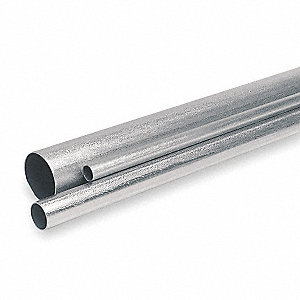
\includegraphics[width=0.25\textwidth,height=\textheight]{/Users/davidlapuma/Dropbox/CTT_Git/ctt_documentation/images/EMT.png}

\hypertarget{building-a-mast-for-your-sensorstation}{%
\subsubsection{Building a mast for your
SensorStation}\label{building-a-mast-for-your-sensorstation}}

\textbf{We don't recommend PVC} because it moves in the wind, becomes
brittle, and will snap over time. EMT can be painted if you would like
them camouflaged.

The conduit can be attached to a tripod, mounted directly into the
ground, or onto a building or other structure. The Nodes and
SensorStations are then attached to the conduit. The diameter of the
conduit is typically 1'' for the top mast section of the SensorStation
(the section to which the antennas are attached; light green in the
picture below).

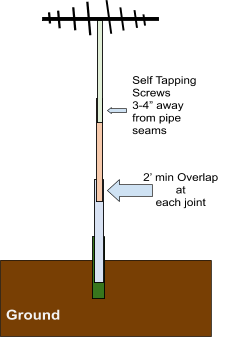
\includegraphics[width=0.25\textwidth,height=\textheight]{/Users/davidlapuma/Dropbox/CTT_Git/ctt_documentation/images/SSinstall.png}

For every 7 feet of height the base section will increase in diameter by
¼''. For example, in the picture above, a 15 foot mast will have a 1''
section (light green) inserted into a 1 ¼'' (orange) and then into a 1
½'' (blue). If the conduit is inserted into the ground, the 1 ½''
conduit should be inserted into a 4' section of 2'' pipe (dark green).
The pipe in the ground is cut in half, the bottom flattened slightly
with sledge hammer to keep soil from entering when it is driven into the
ground. A block of wood can be used to pound the pipe into the ground to
prevent bending the pipe. If the antenna mast is shorter, the next size
up gets driven into the ground (1/ ¼''). Note that standard EMT conduit
does eventually rust, however it will remain very strong for 6-10 years.

If desired, stainless conduit can be purchased, however it is much more
expensive, but \textbf{recommended if you are in an area that receives
high winds}. It is crucial to overlap each section of pipe by at least 2
feet. \textbf{Self tapping screws} are used to hold pipes together, but
should not be used within 3-4'' of the end of the pipes and/or seams.
The chart below should help with what is needed for your setup per
SensorStation.

\begin{longtable}[]{@{}cccc@{}}
\toprule
\begin{minipage}[b]{0.19\columnwidth}\centering
Total Approx Mast Ht.\strut
\end{minipage} & \begin{minipage}[b]{0.23\columnwidth}\centering
EMT Needed for mast (10')\strut
\end{minipage} & \begin{minipage}[b]{0.24\columnwidth}\centering
Ground Section Needed (4')\strut
\end{minipage} & \begin{minipage}[b]{0.22\columnwidth}\centering
Coax Length Per Antenna\strut
\end{minipage}\tabularnewline
\midrule
\endhead
\begin{minipage}[t]{0.19\columnwidth}\centering
7'\strut
\end{minipage} & \begin{minipage}[t]{0.23\columnwidth}\centering
1"\strut
\end{minipage} & \begin{minipage}[t]{0.24\columnwidth}\centering
1 1/4"\strut
\end{minipage} & \begin{minipage}[t]{0.22\columnwidth}\centering
min 10ft\strut
\end{minipage}\tabularnewline
\begin{minipage}[t]{0.19\columnwidth}\centering
15'\strut
\end{minipage} & \begin{minipage}[t]{0.23\columnwidth}\centering
1'',1 ¼''\strut
\end{minipage} & \begin{minipage}[t]{0.24\columnwidth}\centering
1 ½''\strut
\end{minipage} & \begin{minipage}[t]{0.22\columnwidth}\centering
min 20'\strut
\end{minipage}\tabularnewline
\begin{minipage}[t]{0.19\columnwidth}\centering
23'\strut
\end{minipage} & \begin{minipage}[t]{0.23\columnwidth}\centering
1'', 1 ¼'', 1 ½''\strut
\end{minipage} & \begin{minipage}[t]{0.24\columnwidth}\centering
2''\strut
\end{minipage} & \begin{minipage}[t]{0.22\columnwidth}\centering
min 25'\strut
\end{minipage}\tabularnewline
\begin{minipage}[t]{0.19\columnwidth}\centering
28'\strut
\end{minipage} & \begin{minipage}[t]{0.23\columnwidth}\centering
1'', 1 ¼'', 1 ½''\strut
\end{minipage} & \begin{minipage}[t]{0.24\columnwidth}\centering
2''- Use full 10'\strut
\end{minipage} & \begin{minipage}[t]{0.22\columnwidth}\centering
min 30'\strut
\end{minipage}\tabularnewline
\bottomrule
\end{longtable}

\textbf{\emph{Masts higher than 28' not recommended with standard
free-standing EMT conduit. Guy wires and/or scaffold or tripod masts are
other options for higher towers.}}

\hypertarget{mounting-nodes}{%
\subsubsection{Mounting Nodes}\label{mounting-nodes}}

Nodes are typically attached to the top of a ¾'' piece of EMT. The
clamps shown below come standard with the nodes and accept ¾ or 1''
conduit.

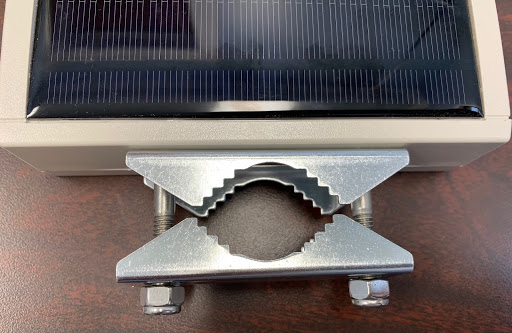
\includegraphics[width=0.25\textwidth,height=\textheight]{/Users/davidlapuma/Dropbox/CTT_Git/ctt_documentation/images/nodeClamp.jpg}

A 7/16'' socket is used to tighten the clamp bolts. The EMT is typically
driven into the ground approximately 2 feet. The height of the nodes can
be changed depending on the project, but for best results should be
consistent within a study site. We recommend 8' for most setups, see
below for pictures of the node setup in the field. If you choose an
alternate mounting method, care should be taken that they are secure. If
they are mounted on anything that sways greatly with the wind, the
readings won't be consistent.

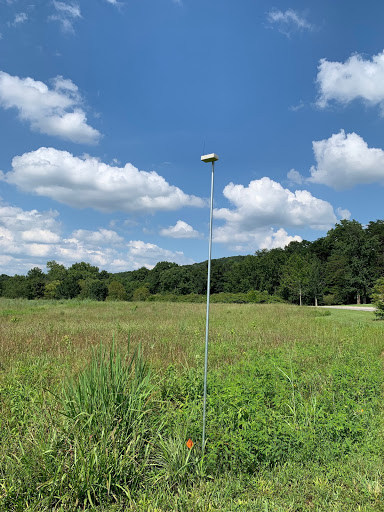
\includegraphics[width=0.25\textwidth,height=\textheight]{/Users/davidlapuma/Dropbox/CTT_Git/ctt_documentation/images/nodeBernh.jpg}
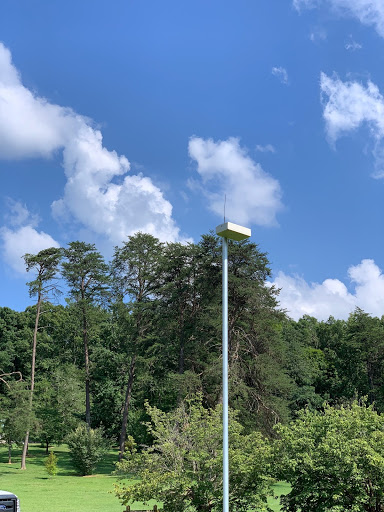
\includegraphics[width=0.25\textwidth,height=\textheight]{/Users/davidlapuma/Dropbox/CTT_Git/ctt_documentation/images/NodeBernh2.jpg}

\textbf{Note:} \textbf{\emph{Nodes purchased in 2020 and beyond have a
built-in GPS. Prior to 2020 you must take accurate GPS readings and
record that data with the Node ID in order to run post-hoc localization
analyses.}}

\hypertarget{node-placement}{%
\subsection{Node Placement}\label{node-placement}}

Setting up the CTT Nodes is typically done in a grid in your study site.
It is not imperative that they are exactly in a grid, but the closer you
can set them up in a grid, the more accurate positioning you will get
from the tags. In sites where this is not practical, you can simply set
them up where you can, 100-300m apart, and record GPS of the Node
locations. Even in a grid setup, it is best practice to take GPS
coordinates whether or not they differ from the layout.

\hypertarget{sensorstation-placement}{%
\subsection{SensorStation Placement}\label{sensorstation-placement}}

The CTT IoW SensorStation may be placed anywhere within range of the
farthest node, which is typically 1-1.5km (although higher placement of
SensorStation antennas, and clear line-of-sight between stations and
nodes, can achieve longer detection distances). See the next section on
SensorStation Configuration and Antenna Detail for more details on this.
It is recommended to place the SensorStation antennas at least 2 meters
high. The higher the antennas, the better range you will get.

\hypertarget{sensorstation-configuration-and-antenna-detail}{%
\subsection{SensorStation Configuration and Antenna
Detail}\label{sensorstation-configuration-and-antenna-detail}}

The standard configuration for the CTT SensorStation allows for
receiving data on \emph{five 434MHz} radio ports simultaneously. These
can be configured to either record signals from LifeTags/PowerTags and
ES-200 GPS loggers (hereafter ``tags''), or to collect data from CTT
Nodes. \emph{Tags and Nodes cannot be picked up on the same channel
simultaneously}, and how you configure your station depends depends on
your study goals. The number of channels necessary on a SensorStation
depends on the number of Nodes, whether you want to detect
tags/transmitters and/or Nodes directly with the SensorStation, and the
distance the Nodes are from the SensorStation.There is no hard limit to
the number of nodes that can be detected by a single SensorStation, but
it's best to keep that number around 50 or less. \emph{Distance to the
SensorStation will usually be the limiting factor for the number of
nodes detectable by a single SensorStation.}

Two types of antennas are commonly used with the SensorStation:
\emph{Omnidirectional} and \emph{Yagi}. \emph{Omnidirectional antennas}
efficiently receive energy in a \emph{horizontal plane 360 degrees
around the SensorStation}. Omnidirectional antennas typically do not
have as great a range as Yagis, but a benefit is the 360 degree
detection, and great detection of tags and nodes that are near the
station.

\textbf{Note: Whereas in the past we have recommended specific
polarization for omnidirectional antennas picking up Nodes vs.~Tags, in
our testing we have found the difference negligible and find vertical
omni antennas to be much simpler and less expensive for a greater value
over horizontally polarized omnis.}

\emph{Yagis are directional antennas} used to detect tags and nodes in a
specific direction from the SensorStation. They \emph{typically have a
30-60 degree detection range that extends away from the SensorStation}.
For that reason typically 2-4 antennas are used, one pointed in each
cardinal direction, or two pointed in opposite directions and used to
make a ``fence''. Yagis can also be used to pick up Nodes that are
farther away from the SensorStation.

While there are many antennas to choose from, these are a few that we
can recommend from experience:

\begin{itemize}
\tightlist
\item
  Omni-directional

  \begin{itemize}
  \tightlist
  \item
    \href{https://www.data-alliance.net/antenna-433mhz-5dbi-omnidirectional-fiberglass-w-n-male-vhf-uhf-marine/}{Data
    Alliance A433O5}

    \begin{itemize}
    \tightlist
    \item
      and you'll need
      \href{https://www.data-alliance.net/l-mount-for-antenna-pole-or-wall-mount-hole-for-n-female-or-rp-sma/}{this
      bracket}
    \item
      and
      \href{https://www.data-alliance.net/n-type-female-to-female-coupler-adapter-w-o-ring-weatherproof-bulkhead/}{this
      adapter}
    \end{itemize}
  \end{itemize}
\item
  Yagi

  \begin{itemize}
  \tightlist
  \item
    \href{https://www.m2inc.com/FG4406SS}{M2Inc 440-6SS}
  \item
    \href{https://www.mouser.com/ProductDetail/Laird-Connectivity/YS4306?qs=EU6FO9ffTwelQ7\%2FXOHiHew\%3D\%3D}{Laird
    YS4306}
  \item
    \href{https://www.hamradio.com/detail.cfm?pid=H0-005816}{Diamond
    A430S10}
  \item
    \href{https://www.dxengineering.com/parts/dmn-a430s15}{Diamond
    A430S15} *for specialized applications where longer-range is
    required
  \end{itemize}
\end{itemize}

\emph{\textbf{Whatever you choose, make sure you get the proper coaxial
end to connect your antenna to your SensorStation!}}

\hypertarget{connecting-antennas-to-your-sensorstation}{%
\subsubsection{Connecting antennas to your
SensorStation}\label{connecting-antennas-to-your-sensorstation}}

To connect antennas to your SensorStation you will need coaxial cable
(we recommend LMR-400 or better) with the proper ends to connect to the
antenna (manufacturer specific) and your SensorStation. If connecting
directly to the board, each 434MHz radio has a \textbf{SMA Female} port,
so your coaxial will require an \textbf{SMA Male} connector.

If connecting to our NEMA case, your coaxial will need a \textbf{Type N
Male connector}.

If connecting an antenna for a different frequency, such as 166MHz, you
will need to attach your Software Defined Radio (SDR) to one of the USB
ports and your coaxial cable to the SMA connector on the SDR. Note that
any 166MHz radios will only show up in the SensorGnome section of the
Web Interface (see \textbf{Sensor Station Web Interface}).

\hypertarget{mounting-the-antennas}{%
\subsubsection{Mounting the antennas}\label{mounting-the-antennas}}

Antennas are attached to the EMT conduit with the clamps that come with
the antennas. If you have a setup that uses 4 yagis, than you will
attach the yagis to a 4 or 5-way mounting ``hat'' you can purchase via
online retailers. Once the antennas are on EMT, attach the coax and wrap
the connection with coax tape. Run down the poles to where it will
attach to the SensorStation. You can use zip ties to secure the coax to
poles where needed. Make sure you have enough coax to form a drip loop
for each connection.

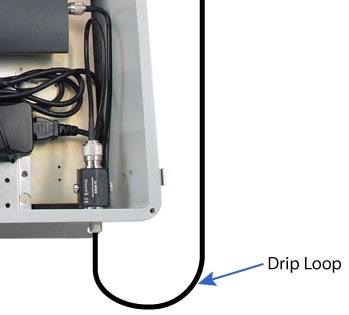
\includegraphics[width=0.25\textwidth,height=\textheight]{/Users/davidlapuma/Dropbox/CTT_Git/ctt_documentation/images/diagram_drip-loop.jpg}

\hypertarget{placing-your-sensorstation}{%
\subsubsection{Placing your
SensorStation}\label{placing-your-sensorstation}}

The SensorStation can be placed inside a building, or fastened to the
pole or building, etc. It should either be close to the ground for easy
access, or have an ethernet cable run down to an accessible location.

\hypertarget{powering-your-sensorstation}{%
\section{Powering your
SensorStation}\label{powering-your-sensorstation}}

The SensorStation can be connected directly to a 12V DC power source,
via a charge controller, or to an AC to DC power supply which can then
be plugged directly into your standard AC power source. In many cases,
though, SensorStations are deployed remotely and are in need of a remote
power supply such as a solar charged deep-cycle marine battery. A
typical setup would be a 50-100W solar panel connected to a charge
controller. The charge controller typically has 3 ports. The 3 ports are
1.) Solar panel 2.) 12V battery 3.) Accessory/Device/consumer, which, in
this case, is your SensorStation. That line goes into the green
\emph{Power In} terminal on the SensorStation board. The positive and
negative wire ports are labeled on the board, and to insert the wire
simply loosen the set screws on the top, and slide the wire leads in to
the holes just under the set screws (see the pictures below; note for V1
stations see the \protect\hyperlink{V1Quickstart}{QuickStart Guide in
Appendix II}).

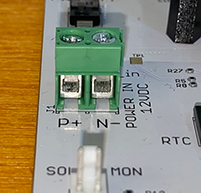
\includegraphics[width=0.2\textwidth,height=\textheight]{/Users/davidlapuma/Dropbox/CTT_Git/ctt_documentation/images/power_out.png}
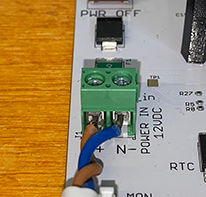
\includegraphics[width=0.2\textwidth,height=\textheight]{/Users/davidlapuma/Dropbox/CTT_Git/ctt_documentation/images/power_in.png}

The ends of the wires that are attached should be tinned with solder for
best results. If you do not have access to a soldering gun, twisting the
ends of the cables tightly will help them slide in cleanly to the power
block.

\hypertarget{monitoring-your-solar-voltage}{%
\subsection{Monitoring your solar
voltage}\label{monitoring-your-solar-voltage}}

If you would like to monitor your solar voltage remotely, you will need
to use the solar monitor connector. it is located above the on/off
switch. Simply run two wires from the solar input of the charge
controller to a two pin connector.

\hypertarget{sensorstation-leds}{%
\section{SensorStation LEDs}\label{sensorstation-leds}}

There are several LED lights on the SensorStation which may assist you
in diagnosing issues. Note that with the introduction of the
SensorStation V2's LCD screen, all diagnoses can be carried out via the
LCD.

\hypertarget{diagnostic-a-green}{%
\subsection{Diagnostic A (green)}\label{diagnostic-a-green}}

\begin{longtable}[]{@{}lll@{}}
\toprule
\begin{minipage}[b]{0.26\columnwidth}\raggedright
LED Behavior\strut
\end{minipage} & \begin{minipage}[b]{0.32\columnwidth}\raggedright
Meaning\strut
\end{minipage} & \begin{minipage}[b]{0.33\columnwidth}\raggedright
Troubleshooting Steps\strut
\end{minipage}\tabularnewline
\midrule
\endhead
\begin{minipage}[t]{0.26\columnwidth}\raggedright
OFF or SOLID\strut
\end{minipage} & \begin{minipage}[t]{0.32\columnwidth}\raggedright
The software has stopped reading data from the radios and writing to the
disk.\strut
\end{minipage} & \begin{minipage}[t]{0.33\columnwidth}\raggedright
Restart your SensorStation.\strut
\end{minipage}\tabularnewline
\begin{minipage}[t]{0.26\columnwidth}\raggedright
Blinking\strut
\end{minipage} & \begin{minipage}[t]{0.32\columnwidth}\raggedright
The software is reading data from the radios and writing that data to
disk.\strut
\end{minipage} & \begin{minipage}[t]{0.33\columnwidth}\raggedright
The system is operating properly.\strut
\end{minipage}\tabularnewline
\bottomrule
\end{longtable}

\hypertarget{diagnostic-b-red}{%
\subsection{Diagnostic B (red)}\label{diagnostic-b-red}}

\begin{longtable}[]{@{}lll@{}}
\toprule
\begin{minipage}[b]{0.26\columnwidth}\raggedright
LED Behavior\strut
\end{minipage} & \begin{minipage}[b]{0.32\columnwidth}\raggedright
Meaning\strut
\end{minipage} & \begin{minipage}[b]{0.33\columnwidth}\raggedright
Troubleshooting Steps\strut
\end{minipage}\tabularnewline
\midrule
\endhead
\begin{minipage}[t]{0.26\columnwidth}\raggedright
ON\strut
\end{minipage} & \begin{minipage}[t]{0.32\columnwidth}\raggedright
Indicates that the SensorStation has established a point-to-point
protocol (PPP) connection between the network and the on-board
modem.\strut
\end{minipage} & \begin{minipage}[t]{0.33\columnwidth}\raggedright
The SensorStation checks for the connection every second. The PPP
connection is just the layer that allows the modem to communicate to the
network \textbf{if it is on}, but doesn't always indicate that a
connection is working (such as in the case of a weak signal)\strut
\end{minipage}\tabularnewline
\begin{minipage}[t]{0.26\columnwidth}\raggedright
OFF\strut
\end{minipage} & \begin{minipage}[t]{0.32\columnwidth}\raggedright
Indicates that the SensorStation modem is not connected to the
network.\strut
\end{minipage} & \begin{minipage}[t]{0.33\columnwidth}\raggedright
If there is no modem on the SensorStation this would be the typical
state and behavior. If a modem exists but this behavior continues, it
indicates that the modem is unable to secure a connection to the
network.\strut
\end{minipage}\tabularnewline
\bottomrule
\end{longtable}

\hypertarget{gsm-cellular-led-blue}{%
\subsection{GSM Cellular LED (blue)}\label{gsm-cellular-led-blue}}

The blue LED by the cellular module, labeled D9, is called the Netlight.
The Netlight blinks differently, depending on the modem state. You can
use this blink rate to identify if your SensorStation is connected to
the Internet or unable to connect.

\begin{longtable}[]{@{}lll@{}}
\toprule
\begin{minipage}[b]{0.26\columnwidth}\raggedright
LED Behavior\strut
\end{minipage} & \begin{minipage}[b]{0.32\columnwidth}\raggedright
Meaning\strut
\end{minipage} & \begin{minipage}[b]{0.33\columnwidth}\raggedright
Troubleshooting Steps\strut
\end{minipage}\tabularnewline
\midrule
\endhead
\begin{minipage}[t]{0.26\columnwidth}\raggedright
OFF\strut
\end{minipage} & \begin{minipage}[t]{0.32\columnwidth}\raggedright
The modem is not currently powered on.\strut
\end{minipage} & \begin{minipage}[t]{0.33\columnwidth}\raggedright
Check to make sure the Raspberry Pi is running.\strut
\end{minipage}\tabularnewline
\begin{minipage}[t]{0.26\columnwidth}\raggedright
Moderate blinking (5 times per second)\strut
\end{minipage} & \begin{minipage}[t]{0.32\columnwidth}\raggedright
The modem is searching for a signal and is not yet connected to a
network.\strut
\end{minipage} & \begin{minipage}[t]{0.33\columnwidth}\raggedright
Wait a minute or two for the modem to find a signal. If it continues to
blink, try using an external antenna or moving the SensorStation to a
better location. Also, be sure that your SensorStation has a data plan
and is activated.\strut
\end{minipage}\tabularnewline
\begin{minipage}[t]{0.26\columnwidth}\raggedright
Slow blinking (once every 2 seconds)\strut
\end{minipage} & \begin{minipage}[t]{0.32\columnwidth}\raggedright
The modem is connected to the network but is idle.\strut
\end{minipage} & \begin{minipage}[t]{0.33\columnwidth}\raggedright
\strut
\end{minipage}\tabularnewline
\begin{minipage}[t]{0.26\columnwidth}\raggedright
Fast blinking (8 times per second)\strut
\end{minipage} & \begin{minipage}[t]{0.32\columnwidth}\raggedright
The modem is connected to the network and is transferring data.\strut
\end{minipage} & \begin{minipage}[t]{0.33\columnwidth}\raggedright
\strut
\end{minipage}\tabularnewline
\bottomrule
\end{longtable}

\hypertarget{sensorstation-navigation-buttons}{%
\section{SensorStation Navigation
Buttons}\label{sensorstation-navigation-buttons}}

The SensorStation features 4 navigation buttons labeled \texttt{UP},
\texttt{DN}, \texttt{BACK} and \texttt{SELECT}. They are typically used
with the SensorStation software to navigate the LCD display.

\hypertarget{technical-description}{%
\subsection{Technical Description}\label{technical-description}}

These buttons are directly wired to the Compute Module's GPIO lines
BCM4, 5, 6, and 7. You will need to enable pullups on these lines to use
these buttons.

\hypertarget{sensorstation-lcd-menu}{%
\section{SensorStation LCD Menu}\label{sensorstation-lcd-menu}}

\begin{itemize}
\tightlist
\item
  \texttt{File\ Transfer}

  \begin{itemize}
  \tightlist
  \item
    \texttt{Mount\ USB} - mounts a properly formatted (FAT-32 or MS-DOS)
    USB drive to the SensorStation.
  \item
    \texttt{Unmount\ USB} - un-mounts a properly formatted (FAT-32 or
    MS-DOS) USB drive from the SensorStation. This should be used before
    removing a USB drive from your SensorStation.
  \item
    \texttt{Download} - downloads all data on the SensorStation to the
    mounted USB drive.
  \item
    \texttt{Get\ WiFi} - loads WiFi credentials from JSON document
    located in \texttt{wifi} folder on mounted USB drive (see
    \textbf{Connecting your SensorStation to a local wireless network}
    below).
  \end{itemize}
\item
  \texttt{System}

  \begin{itemize}
  \tightlist
  \item
    \texttt{About}

    \begin{itemize}
    \tightlist
    \item
      \texttt{Image} - provides the image creation date, and the date of
      last update.
    \item
      \texttt{Ids} - displays the \texttt{System\ Ids} which include the
      \texttt{SensorStation\ serial\ number} \texttt{SIM\ number}
      \texttt{Broadcom\ chip\ id} and
      \texttt{Raspberry\ Pi\ serial\ number}
    \item
      \texttt{Memory} - displays the amount of used memory and the total
      disk size.
    \item
      \texttt{Uptime} - Displays the total up time since the station was
      last rebooted.
    \end{itemize}
  \item
    \texttt{QAQC} - this is an internal function which will eventually
    be useful to the end-user but not as of this printing.
  \item
    \texttt{Time} - The three clocks on the SensorStation, refreshing
    every two seconds. \texttt{r}eal time clock, \texttt{g}ps clock and
    \texttt{s}ystem clock.
  \item
    \texttt{Restart} - Triggers a system restart.
  \end{itemize}
\item
  \texttt{Network}

  \begin{itemize}
  \tightlist
  \item
    \texttt{Cellular}

    \begin{itemize}
    \tightlist
    \item
      \texttt{Ids} - - Displays the SIM ID, the IMEI, and the name of
      the Modem
    \item
      \texttt{Carrier} - Displays the cellular carrier name and signal
      strength of the connection, refreshing every 2 seconds. This may
      be useful when troubleshooting problematic GSM connections, and
      aiming an external cellular antenna (not included).
    \end{itemize}
  \item
    \texttt{Ping} - This will ping a known web address to determine
    whether an internet connection is present. If present, it will
    return \textbf{connected}.
  \item
    \texttt{Hostname} - Typically this is \texttt{sensorstation.local}
    and can be used to reach your station when it is connected to WiFi,
    a local network via Ethernet, or directly to a computer via
    Ethernet. Once connected, simply navigate to
    \url{http://sensorstation.local} in your web browser to access the
    SensorStation interface.
  \item
    \texttt{IP\ Address} - Displays the port of connection and IP
    address assigned to the SensorStation. You can use the IP address to
    connect to your SensorStation using the same process outlined above
    under \texttt{Hostname}. For example, if the IP Address was
    10.1.10.17, typing \texttt{http://10.1.10.17} into your web
    browser's URL field would bring up the SensorStation web interface.
  \end{itemize}
\item
  \texttt{Server} - causes the SensorStation to force a check-in to the
  CTT hardware server. Requires that the SensorStation is connected to
  the internet via either GSM, WiFi or Ethernet. Note that this process
  may take a long time depending on connection speed and/or amount of
  data being sent/received.
\item
  \texttt{Power} - Provides voltages for \texttt{Battery} (which
  represents whatever power source is connected to your SensorStation),
  \texttt{RTC} or Real Time Clock, the coin cell battery on the board,
  and \texttt{Solar} if you have connected a solar monitoring cable from
  the charge controller to the SensorStation board.
\item
  \texttt{Temperature} - Provides the temperature of the SensorStation
  board. Note temperature will usually be higher than ambient when the
  board is powered.
\item
  \texttt{Location} - provides the Lat/Long for the SensorStation from
  the on-board GPS.
\item
  \texttt{LED} - allows you to select various LED and toggle them
  \texttt{on}, \texttt{off} or \texttt{blink}.

  \begin{itemize}
  \tightlist
  \item
    \texttt{Diagnostic\ A} - this LED represents the connectivity to CTT
    servers.

    \begin{itemize}
    \tightlist
    \item
      \texttt{On} - Turns the LED \texttt{on}, if current state is
      \texttt{off}.
    \item
      \texttt{Off} - Turns the LED \texttt{off}, if current state is
      \texttt{on}.
    \item
      \texttt{Blink} - Blinks the LED once.
    \end{itemize}
  \item
    \texttt{Diagnostic\ B} - this LED represents the connectivity to the
    cellular network (if a cell modem is installed).

    \begin{itemize}
    \tightlist
    \item
      \texttt{On} - Turns the LED \texttt{on}, if current state is
      \texttt{off}.
    \item
      \texttt{Off} - Turns the LED \texttt{off}, if current state is
      \texttt{on}.
    \item
      \texttt{Blink} - Blinks the LED once.
    \end{itemize}
  \item
    \texttt{GPS} - this green LED has three states: Solid (3D Fix),
    Blinking 2x/second (2D fix), Blinking 5x/second (No Fix).

    \begin{itemize}
    \tightlist
    \item
      \texttt{On} - Turns the LED \texttt{on}, if current state is
      \texttt{off}.
    \item
      \texttt{Off} - Turns the LED \texttt{off}, if current state is
      \texttt{on}.
    \item
      \texttt{Blink} - Blinks the LED once.
    \end{itemize}
  \end{itemize}
\end{itemize}

\begin{center}\rule{0.5\linewidth}{0.5pt}\end{center}

\hypertarget{downloading-your-data-via-a-usb-thumb-drive}{%
\section{Downloading your data via a USB Thumb
Drive}\label{downloading-your-data-via-a-usb-thumb-drive}}

\begin{enumerate}
\def\labelenumi{\arabic{enumi}.}
\tightlist
\item
  Insert a properly formatted (currently only MS DOS or Fat32 formatting
  is supported) USB thumb drive in one of the seven USB ports.
\item
  Navigate to \texttt{File\ Transfer\ \textgreater{}\ Mount\ USB} and
  press the \texttt{SELECT} button. You should see a confirmation
  message saying \texttt{USB\ Mount:success}.
\item
  Use the \texttt{BACK} button to go up to the \texttt{File\ Transfer}
  menu, and select \texttt{Download}. A successful download will be
  followed by a success message.
\item
  Use the \texttt{Back} button to go up to the \texttt{File\ Transfer}
  menu and select \texttt{Unmount\ USB}. Once you receive the success
  message you may remove the USB drive from the SensorStation which will
  now contain a copy of all the files from the station.
\end{enumerate}

\hypertarget{whats-in-the-folder}{%
\subsection{What's in the folder?}\label{whats-in-the-folder}}

On your USB drive you will find several files\ldots{}

\begin{itemize}
\tightlist
\item
  \textbf{gps} files - these contain the GPS coordinates of the
  SensorStation's location

  \begin{itemize}
  \tightlist
  \item
    \texttt{recorded\ at} - time/date stamp for the time the row was
    written to the file (UTC)
  \item
    \texttt{gps\ at} - time/date stamp for the instantaneous time of the
    last GPS fix (UTC)
  \item
    \texttt{latitude} - in decimal degrees
  \item
    \texttt{longitude} - in decimal degrees
  \item
    \texttt{altitude} - in meters
  \item
    \texttt{quality}

    \begin{itemize}
    \tightlist
    \item
      \texttt{1} - No fix.
    \item
      \texttt{2} - 2D fix. Medium quality.
    \item
      \texttt{3} - 3D fix. Highest quality.
    \end{itemize}
  \item
    \texttt{mean\ lat} - in decimal degrees, based on n fixes.
  \item
    \texttt{mean\ lng} - in decimal degrees, based on n fixes.
  \item
    \texttt{n\ fixes} - number of fixes used to calculate mean lat and
    lng.
  \end{itemize}
\item
  \textbf{log} files

  \begin{itemize}
  \tightlist
  \item
    \texttt{msg\ at} - The date/time stamp of the message.
  \item
    \texttt{msg} - The text string of the message at that time.
  \end{itemize}
\item
  \textbf{raw-data} files

  \begin{itemize}
  \tightlist
  \item
    \texttt{Time} - Date/time stamp of the data point in
    \texttt{YYYY-MM-DD\ HH:MM:SS}.
  \item
    \texttt{RadioID} - The ID of the radio from which the data point was
    collected. These correspond to the Radios L1 - L5 on your
    SensorStation (standard 434MHz radios).
  \item
    \texttt{TagID} - The 8-digit ID of the tag that was detected. Note
    that for tags with 10-digit IDs (e.g.~V2 LifeTag), this will be
    represented by the first 8 digits in that ID.
  \item
    \texttt{TagRSSI} - The signal strength of the transmission, measured
    in Decibels (DB). Values. closer to zero represent stronger signals.
    Values below -110 DB are typically not useful for estimating
    distance.
  \item
    \texttt{NodeId} - The unique ID of the node from which the
    transmission was received.
  \item
    \texttt{Validated} - Binary value that indicates whether the CRC
    value corroborated the unique tag ID. 0 = invalidated; 1 =
    validated. \textbf{MORE EXPLANATION HERE}
  \end{itemize}
\end{itemize}

And two folders:

\begin{itemize}
\tightlist
\item
  \texttt{SGData} - contains any 166MHz data collected by your station.
\item
  \texttt{uploaded} - contains any 434MHz data that has been previously
  uploaded to CTT servers.
\end{itemize}

\begin{center}\rule{0.5\linewidth}{0.5pt}\end{center}

\hypertarget{connecting-to-your-sensorstation-web-interface}{%
\section{Connecting to your SensorStation Web
Interface}\label{connecting-to-your-sensorstation-web-interface}}

\hypertarget{connecting-via-ethernet-cable}{%
\subsection{Connecting via Ethernet
Cable}\label{connecting-via-ethernet-cable}}

\hypertarget{before-you-get-started-you-will-need}{%
\subsubsection{Before you get started you will
need\ldots{}}\label{before-you-get-started-you-will-need}}

\begin{itemize}
\tightlist
\item
  2 USB to Ethernet adapters (we recommend:
  \url{https://tinyurl.com/yc6llze4})
\item
  An Ethernet cable
\end{itemize}

\hypertarget{making-the-connection}{%
\subsubsection{Making the Connection}\label{making-the-connection}}

\begin{enumerate}
\def\labelenumi{\arabic{enumi}.}
\tightlist
\item
  Connect each end of the Ethernet cable to the two
  USB-\textgreater Ethernet adapters.
\item
  Plug one USB end of an adapter into any of the USB ports on your
  SensorStation.
\item
  Plug the USB end of the second adapter into your computer and wait up
  to two minutes to allow the SensorStation to acquire the IP address
  from your computer.
\item
  You can test this connection through several diagnostics in the LCD
  menu. * \texttt{Network\ \textgreater{}\ Ping} will indicate a
  connection. * \texttt{Network\ \textgreater{}\ IP\ Address} will
  display a valid IP address.
\item
  Open a web browser on your computer, and put the IP address from Step
  5 into the URL window of the browser. The web interface should appear.
\end{enumerate}

\emph{If for some reason you are unable to connect after Step 3, try
restarting both the SensorStation and your computer and continue to Step
4.}

\begin{center}\rule{0.5\linewidth}{0.5pt}\end{center}

\hypertarget{connecting-via-local-wireless-network-on-v1-sensorstation-but-also-works-on-v2}{%
\subsection{\texorpdfstring{Connecting via Local Wireless Network on
\textbf{V1 SensorStation} (but also works on
V2)}{Connecting via Local Wireless Network on V1 SensorStation (but also works on V2)}}\label{connecting-via-local-wireless-network-on-v1-sensorstation-but-also-works-on-v2}}

\hypertarget{before-you-get-started-you-will-need-1}{%
\subsubsection{Before you get started you will
need\ldots{}}\label{before-you-get-started-you-will-need-1}}

\begin{itemize}
\tightlist
\item
  WiFi adapter Like this one:
  \url{https://store.celltracktech.com/products/wifi-usb-adapter-add-on-for-sensorstation-v2}.
\item
  2 USB to Ethernet adapters (we recommend:
  \url{https://tinyurl.com/yc6llze4})
\item
  An Ethernet cable
\end{itemize}

\hypertarget{gather-important-information}{%
\subsubsection{Gather important
information}\label{gather-important-information}}

\begin{enumerate}
\def\labelenumi{\arabic{enumi}.}
\tightlist
\item
  Take note of the \textbf{Wifi name} and \textbf{password} for the
  network you want to link with your SensorStation.
\item
  Connect to your SensorStation via the Ethernet cable (see above
  section for details)
\item
  Open a terminal window (Terminal on Mac, Command Prompt on PC) and
  issue the following command:
\end{enumerate}

\texttt{arp\ -a}

This will give you a list of all of the connected devices.

\begin{enumerate}
\def\labelenumi{\arabic{enumi}.}
\setcounter{enumi}{3}
\tightlist
\item
  Take a screenshot of this list, or jot them down. You'll need this
  later.
\end{enumerate}

\hypertarget{ssh-into-the-pi-to-update-the-connectivity-settings}{%
\subsubsection{SSH into the Pi to update the connectivity
settings}\label{ssh-into-the-pi-to-update-the-connectivity-settings}}

\begin{enumerate}
\def\labelenumi{\arabic{enumi}.}
\setcounter{enumi}{4}
\tightlist
\item
  Type the following:
\end{enumerate}

\texttt{ssh\ pi@xxx.xxx.xxx.xxx} (where the x's represent your
SensorStation IP address)

\begin{enumerate}
\def\labelenumi{\arabic{enumi}.}
\setcounter{enumi}{5}
\item
  Answer \texttt{yes} to any dialogues, and when prompted for the
  password, the default password is \texttt{raspberry}.
\item
  At this point you should be in the Secure Shell within your Raspberry
  Pi. From here issue the following command:
\end{enumerate}

\texttt{sudo\ raspi-config}

\begin{enumerate}
\def\labelenumi{\arabic{enumi}.}
\setcounter{enumi}{7}
\item
  From the config dialogue use the DOWN ARROW to select
  \texttt{Network\ Options}
\item
  Then choose
  \texttt{N2\ Wireless\ LAN\ -\ Enter\ SSID\ and\ PASSPHRASE}
\item
  From there enter your \texttt{wireless\ network\ ID\ (SSID)} and the
  \texttt{password/phrase} for your WiFi network.
\item
  \texttt{Save} and \texttt{exit}.
\item
  Close the terminal.
\item
  Restart your SensorStation.
\end{enumerate}

\hypertarget{wirelessly-connect-to-your-sensorstation}{%
\subsubsection{Wirelessly connect to your
SensorStation}\label{wirelessly-connect-to-your-sensorstation}}

Once your SensorStation reboots, it should automatically connect to the
existing wireless network, and you will be able to reach the station via
any device on the same wireless network. Note that the IP address for
your station will have changed- but in most cases you can use the
\texttt{Hostname} to connect, or you can run \texttt{arp\ -a} from the
command-line to search for your station's new IP address.

\begin{enumerate}
\def\labelenumi{\arabic{enumi}.}
\setcounter{enumi}{13}
\tightlist
\item
  Open up a web browser and try and connect by typing the following
  Hostname into the address bar:
\end{enumerate}

\emph{For V1 SensorStations:} \texttt{raspberrypi.local}

\emph{For V2 SensorStations:} \texttt{sensorstation.local}

\begin{enumerate}
\def\labelenumi{\arabic{enumi}.}
\setcounter{enumi}{14}
\tightlist
\item
  If that doesn't work, open up another terminal window and type:
\end{enumerate}

\texttt{arp\ -a}

Look for a change in the connected device IP addresses. You should be
able to identify a new one that wasn't there the last time. This is your
SensorStation. You can now type that IP address in the web address bar
and should see the SensorStation dialogue pop up.

\hypertarget{connecting-via-local-wireless-network-on-v2-sensorstation}{%
\subsection{\texorpdfstring{Connecting via Local Wireless Network on
\textbf{V2
SensorStation}}{Connecting via Local Wireless Network on V2 SensorStation}}\label{connecting-via-local-wireless-network-on-v2-sensorstation}}

On the new V2 SensorStation, instead of manually updating the WiFi
credentials via SSH, you can use the \texttt{Get\ WiFi} function
available via the LCD menu to upload a credentials file. Follow the
steps below to learn how.

\hypertarget{before-you-get-started-you-will-need-2}{%
\subsubsection{Before you get started you will
need\ldots{}}\label{before-you-get-started-you-will-need-2}}

\begin{itemize}
\tightlist
\item
  WiFi adapter Like this one:
  \url{https://store.celltracktech.com/products/wifi-usb-adapter-add-on-for-sensorstation-v2}.
\item
  Properly formatted USB thumb drive (Fat-32 or MS-DOS formatting
  currently supported).
\item
  A code editor where you can control the programming language and line
  encoding. We recommend the free Visual Studio Code
  (\url{https://code.visualstudio.com}).
\end{itemize}

\hypertarget{creating-the-json-file}{%
\subsubsection{Creating the JSON file}\label{creating-the-json-file}}

\begin{enumerate}
\def\labelenumi{\arabic{enumi}.}
\tightlist
\item
  In your code editor, create a new file and set the \textbf{Language
  Mode} to \texttt{JSON} and the \textbf{End of Line Sequence} to
  \textbf{LF} (for Line Feed).
\item
  Type the following into the file:
\end{enumerate}

\begin{verbatim}
  {
    "ssid":"my_ssid",
    "psk":"my_password" 
  }
\end{verbatim}

\textbf{Make sure you change ``my\_ssid'' to the name of your wifi
network and ``my\_password'' to the password for your wifi network!}

\begin{enumerate}
\def\labelenumi{\arabic{enumi}.}
\setcounter{enumi}{2}
\tightlist
\item
  Save the file and name it \texttt{credentials.json}.
\item
  Create an empty folder on your USB thumb drive called \texttt{wifi}.
\item
  Copy \texttt{credentials.json} file to the \texttt{wifi} folder.
\end{enumerate}

\hypertarget{loading-the-json-file-onto-your-sensorstation}{%
\subsubsection{Loading the JSON file onto your
SensorStation}\label{loading-the-json-file-onto-your-sensorstation}}

\begin{enumerate}
\def\labelenumi{\arabic{enumi}.}
\tightlist
\item
  Make sure your SensorStation is powered on and the menu is visible on
  the LCD screen
\item
  Insert your USB thumb drive into any of the USB ports on your
  SensorStation.
\item
  Using the four buttons right of the LCD screen, navigate to
  \texttt{File\ Transfer\ \textgreater{}\ Mount\ USB} and click the
  \texttt{Select} button.
\item
  You should receive a \texttt{success} message.
\item
  Now navigate to \texttt{File\ Transfer\ \textgreater{}\ Get\ WiFi} and
  click the \texttt{Select} button.
\item
  You should receive a \texttt{success} message.
\item
  Restart your SensorStation.
\item
  After restart, your SensorStation should be connected to your local
  wifi network. You can test this connection through several diagnostics
  in the LCD menu.
\end{enumerate}

\begin{itemize}
\tightlist
\item
  \texttt{Network\ \textgreater{}\ Ping} will indicate a connection.
\item
  \texttt{Network\ \textgreater{}\ IP\ Address} will display a valid IP
  address.
\end{itemize}

\hypertarget{connecting-to-your-wifi-enabled-sensorstation}{%
\subsubsection{Connecting to your wifi-enabled
SensorStation}\label{connecting-to-your-wifi-enabled-sensorstation}}

Once your station has connected to your wifi network, you can connect to
your SensorStation wirelessly via any device on the \textbf{same wifi
network} as the station.

\begin{itemize}
\tightlist
\item
  Connect your computer, tablet or smartphone to the same wifi network
  as your SensorStation.
\item
  open a web browser on your computer, tablet or smartphone and navigate
  to the IP address found via the
  \texttt{Network\ \textgreater{}\ IP\ Address} on your SensorStation's
  LCD screen. Alternatively you can use the name found in
  \texttt{Network\ \textgreater{}\ Hostname}, which is typically
  \texttt{sensorstation.local}.
\end{itemize}

\begin{center}\rule{0.5\linewidth}{0.5pt}\end{center}

\hypertarget{the-sensorstation-web-interface}{%
\section{The SensorStation Web
Interface}\label{the-sensorstation-web-interface}}

\hypertarget{overview}{%
\subsection{Overview}\label{overview}}

The SensorStation Web Interface provides an overview of your station's
operation, including real-time statistics on detections of tags and
nodes, as well as a user interface to change settings, update your
SensorStation, toggle the GSM modem, and reboot the station.

\hypertarget{nodes}{%
\subsection{Nodes}\label{nodes}}

This is a list of Nodes the station has detected since connecting. For
each Node it lists:

\texttt{Node\ ID} \texttt{Last\ Heard} - the time of the last health
report \texttt{Node\ RSSI} - the RSSI of the Node signal in decibels
\texttt{Battery\ Voltage} - the Node's battery voltage, which can be
used to estimate its remaining life. 4.2 V is very full. 3.5 Vis low. 3
V is nearly empty. \texttt{Node\ Firmware\ Version}

\hypertarget{tags}{%
\subsection{Tags}\label{tags}}

This is a list of unique LifeTags that have been detected by your
radios. For each tag it lists

\begin{itemize}
\tightlist
\item
  \texttt{Tag\ ID}
\item
  \texttt{Count} - number of beeps since last page refresh
\item
  \texttt{Alias} - for convenience, a name can be given to a particular
  tag and saved in the browser by hitting the \texttt{Update} button.
  This information is saved in your browser only. Name it whatever you'd
  like. Great for keeping track of particular tags during a test.
\item
  \texttt{“Update”\ Button} - save the name of a particular tag to your
  browser
\item
  \texttt{“Remove”\ Button} - reset the saved name
\end{itemize}

\hypertarget{station}{%
\subsection{Station}\label{station}}

Various information about your SensorStation is stored here.

\begin{itemize}
\item
  \texttt{ID} - the serial number of your SensorStation (the cell
  modem's IMEI)
\item
  \texttt{Compute\ Module\ Serial} - the serial number of your Raspberry
  Pi Compute Module
\item
  \texttt{Module\ Hardware} - the compute module's hardware version
\item
  \texttt{Module\ Revision} - the compute module's hardware revision
\item
  \texttt{Boot\ Count} - the number of times the system has been booted
\item
  \texttt{Total\ Memory} - the amount of RAM currently being used by the
  system
\item
  \texttt{Last\ Boot} - Datetime of last boot
\item
  \texttt{Memory\ Usage} - A pie chart indicating the amount of system
  RAM currently being used.
\item
  \texttt{CPU\ Usage} - A pie chart indicating the amount of processing
  power currently being used.
\item
  \texttt{Tag\ Histogram} - A histogram of tags detected since opening
  the interface. The bars indicate the number of beeps detected.
\item
  \texttt{Time\ Sync\ Stats} - Detailed information of how the system
  time is being retrieved synced (e.g.~from GPS or the internet)
\end{itemize}

\hypertarget{sensorstation-log}{%
\subsection{SensorStation Log}\label{sensorstation-log}}

A log of SensorStation activity. Includes things such as screen updates
and data retrieval flushes.

\hypertarget{gps}{%
\subsection{GPS}\label{gps}}

Information retrieved over GPS: Time, Satellites, Latitude, Longitude,
Altitude. If there is currently no valid fix, these fields will be
blank.

\hypertarget{radios-1-5}{%
\subsection{Radios (1-5)}\label{radios-1-5}}

There is a display box for each Radio port. The boxes will display all
new data from each Radio port as they are detected, informing you of the
following:

\begin{itemize}
\tightlist
\item
  \texttt{Time}
\item
  \texttt{Tag\ ID}
\item
  \texttt{RSSI}
\item
  \texttt{Node}from which it came (if applicable).
\end{itemize}

\hypertarget{radio-configuration}{%
\subsubsection{Radio Configuration}\label{radio-configuration}}

Each of the five 434MHz radios can be individually configured to receive
\texttt{Nodes}, \texttt{Tags\ (FSK)}, or \texttt{OOK\ (legacy\ tags)} by
clicking the corresponding button. On V1 SensorStations this
configuration will only persist until the next webpage refresh unless
you press the ``Save Radio Configuration'' button below, which will save
the configuration permanently to memory. For V2 SensorStations the
setting is automatically saved as soon as you acknowledge the
confirmation popup after clicking the \texttt{Node}, \texttt{Tag} or
\texttt{OOK} buttons for a particular radio. Configurations can be
changed at any time. \textbf{Note that once you have changed the radio
settings, the change is immediately saved and the data will flow from
whichever you changed it to; node or tag, but in order to see the text
description change on the web interface, you will need to refresh the
webpage.}

\texttt{Node} = CTT Nodes Only \texttt{Tag} = CTT LifeTags, PowerTags,
ES-200 and ES-150 GPS tags \texttt{OOK} = Legacy-style LifeTag only for
limited specialized project

\texttt{Clear\ Session\ Data} simply clears the scrolling log of tags
displayed for each radio port. It does not delete any data from system
memory.

\hypertarget{data-management}{%
\subsection{Data Management}\label{data-management}}

The data management section is the interface through which your station
data is retrieved and deleted.

\hypertarget{server-utilities}{%
\subsection{Server Utilities}\label{server-utilities}}

From the Server Utilities section on the web interface, you can now
\texttt{Update\ Your\ SensorStation} to the latest deployment build, as
well as force \texttt{Check\ In} and force \texttt{Upload\ Data} to the
CTT servers.

\textbf{Requirement:}

\begin{itemize}
\tightlist
\item
  Because these buttons require connecting to servers via the internet,
  your SensorStation must be connected to the internet, either via the
  \emph{on-board LTE module}, hardwired via \emph{Ethernet} (this
  includes being connected to a computer via Ethernet which is connected
  to the internet), or wirelessly via a \emph{WiFi adapter}.
\end{itemize}

\hypertarget{updating-your-sensorstation}{%
\subsubsection{Updating your
SensorStation}\label{updating-your-sensorstation}}

\begin{enumerate}
\def\labelenumi{\arabic{enumi}.}
\tightlist
\item
  With the CTT Sensor Station Overview page open in your browser, scroll
  down to \texttt{Server\ Utilities} on the right sidebar.
\item
  Click the button labeled \texttt{Station\ Update}, which will open the
  \texttt{Sensor\ Station\ Software\ Updater} console
\item
  Scroll down below the console window and click on the
  \texttt{Update\ Station} button. This will begin the update process.
  Be aware that the station will be pulling code from five different
  code bases, which may take up to several minutes depending on your
  connection speed.
\item
  When the process is complete, you will receive a
  \texttt{Station\ connection\ disconnected} dialogue. \textbf{This
  indicates that the update is complete} and that the system has
  restarted. You may now click the dialogue to clear it, and then click
  the button at the bottom of the screen to go
  \texttt{Back\ to\ Main\ Interface}.
\end{enumerate}

\hypertarget{station-log}{%
\subsection{Station Log}\label{station-log}}

Allows you to \textbf{download} (\texttt{Download\ Log\ File}) and
\textbf{PERMANENTLY DELETE} (\texttt{Clear\ Log\ File}) the system log
file. Used for informational and debugging purposes.

\hypertarget{ctt-tag-data}{%
\subsection{CTT Tag Data}\label{ctt-tag-data}}

The tag data is divided into \texttt{Current\ Data},
\texttt{Data\ Not\ Uploaded}, and \texttt{Data\ Already\ Uploaded}.
Current Data is data from the last 30 minutes. After 30 minutes, data is
rotated into Data Not Uploaded, which is data beyond the last 30 minutes
which has not yet been uploaded to CTT servers. If there is an internet
connection via cell or ethernet, an upload attempt occurs every 2 hours.
After data is uploaded, it is rotated into
\texttt{Data\ Already\ Uploaded} and will stay there until you
explicitly delete it. The red Delete buttons will \textbf{PERMANENTLY
DELETE} the corresponding data from the SensorStation. An \emph{are you
sure} dialogue will make sure you do not accidentally delete data.

\hypertarget{nanotag-data}{%
\subsection{Nanotag Data}\label{nanotag-data}}

Nanotag Data uses the same scheme as CTT Tag Data, except that currently
data from the last 30 minutes is unavailable from this screen. The
Sensorgnome interface is separately accessible as described below.

\hypertarget{nanotag-data-sensorgnome-interface}{%
\subsubsection{Nanotag Data / Sensorgnome
Interface}\label{nanotag-data-sensorgnome-interface}}

\hypertarget{sensorgnome-interface}{%
\subsection{Sensorgnome Interface}\label{sensorgnome-interface}}

Click the ``Sensorgnome Interface'' button to go to the Sensorgnome
interface.

\hypertarget{sensorgnome-deployment-file}{%
\subsection{Sensorgnome Deployment
File}\label{sensorgnome-deployment-file}}

The Sensorgnome Deployment file can be edited here and saved by clicked
\texttt{Save\ Changes}.

\hypertarget{reboot-button}{%
\subsection{Reboot Button}\label{reboot-button}}

Reboots the system.

\begin{center}\rule{0.5\linewidth}{0.5pt}\end{center}

\hypertarget{troubleshooting}{%
\section{Troubleshooting}\label{troubleshooting}}

\textbf{I get an error when I attempt to mount my USB drive}

\emph{Your USB drive may not be formatted properly}

\textbf{I have successfully mounted my USB drive but when I go to
\texttt{Add\ Wifi} I get an error}

\emph{Either your USB drive is not formatted properly (some formats will
allow you to mount, but not to read the file, such as X-Fat on Mac)}
\textbf{or} \emph{your JSON file is not properly formatted.}

\begin{itemize}
\tightlist
\item
  Verify the following:

  \begin{itemize}
  \tightlist
  \item
    Your file is named \texttt{credentials.json}
  \item
    Your file is in a folder called \texttt{wifi}
  \item
    There is only one folder called \texttt{wifi} on your USB thumb
    drive
  \item
    Your JSON file was created with the End of Line Sequence set to
    \textbf{LF}
  \item
    Your JSON file was properly formatted (see \textbf{\#2} under
    \textbf{Creating the JSON file} above)
  \item
    Note you can always check your code validity by pasting it into this
    website: \url{https://jsonlint.com} and clicking
    \texttt{Validate\ JSON}
  \end{itemize}
\end{itemize}

\begin{center}\rule{0.5\linewidth}{0.5pt}\end{center}

\hypertarget{known-bugs}{%
\section{Known Bugs}\label{known-bugs}}

\begin{enumerate}
\def\labelenumi{\arabic{enumi}.}
\tightlist
\item
  SensorStations without a modem installed will not check in to the CTT
  system.
\end{enumerate}

\begin{center}\rule{0.5\linewidth}{0.5pt}\end{center}

\hypertarget{appendix_1}{%
\section{Appendix I: Leveraging your CTT Infrastructure with
Motus}\label{appendix_1}}


\includegraphics[width=0.1\textwidth,height=\textheight]{/Users/davidlapuma/Dropbox/CTT_Git/ctt_documentation/images/motus-logo.png}

\includegraphics[width=0.1\textwidth,height=\textheight]{/Users/davidlapuma/Dropbox/CTT_Git/ctt_documentation/images/BirdsCanadaLogo.png}

\includegraphics[width=0.15\textwidth,height=\textheight]{/Users/davidlapuma/Dropbox/CTT_Git/ctt_documentation/images/ctt_logo_300DPI.jpg}

\hypertarget{the-motus-wildlife-tracking-system}{%
\subsection{The Motus Wildlife Tracking
System}\label{the-motus-wildlife-tracking-system}}

When tracking wildlife with automated radio telemetry over vast
distances, the challenge of deploying enough receivers to get detections
grows exponentially. To remedy this, data can be shared between all
researchers so that essentially everyone is sharing receivers. This
greatly expands the potential for this technology, but it comes with the
added responsibility of coordinating projects, detection data and
metadata - that's where Motus comes in.

\hypertarget{what-is-motus}{%
\subsection{What is Motus?}\label{what-is-motus}}

The Motus Wildlife Tracking System is an international collaborative
network of researchers that use automated radio telemetry to
simultaneously track hundreds of individuals of numerous species of
birds, bats, and insects. The system enables a community of researchers,
educators, organizations, and citizens to undertake impactful research
and education on the ecology and conservation of migratory animals. When
compared to other technologies, automated radio telemetry currently
allows researchers to track the smallest animals possible, with high
temporal and geographic precision, over great distances.

\hypertarget{how-does-motus-work}{%
\subsection{How does Motus work?}\label{how-does-motus-work}}

The entire philosophy behind Motus is that we're all working together.
At its core, Motus is community science. A community of researchers
around the world conducting research on animals are tracked by a network
of receiving stations maintained by a community of researchers,
organizations, non-profits, governments, and individuals. In order for
this concept to work, the system requires a centralized database and
management system that all participants use. Most importantly, in order
for your tags to be detected on any other station in the network, or for
other project tags to be detected elsewhere, projects, receivers and
tags need to be registered with, and have data processed by Motus.

While any automated telemetry project can operate in isolation,
operating as a Motus project combines the collective impact of local,
regional, and even hemispheric projects into one massive collaborative
effort that expands the scale and scope of everyone's work and maximizes
the use of scarce research dollars. It also makes data available and
more useful for future projects, collaborative endeavors and large-scale
meta analyses.

\hypertarget{whats-the-cost}{%
\subsection{What's the cost?}\label{whats-the-cost}}

There is NO cost to register your project and receivers to the Motus
network and contribute your data. Tags registered to the network are
charged a nominal fee to support data processing and ongoing maintenance
and development of the system. See the collaboration policy and fee
schedule for more information.

\hypertarget{data-ownershipprivacy}{%
\subsection{Data Ownership/Privacy}\label{data-ownershipprivacy}}

The collaborative nature of Motus relies on a certain level of
transparency with respect to data. While basic project and tag summary
information is made publicly available, researchers have the ability to
customize data accessibility and keep their project and data private if
necessary. See the collaboration policy for more information.

\begin{center}\rule{0.5\linewidth}{0.5pt}\end{center}

\hypertarget{how-to-join-motus-in-3-or-5-easy-steps}{%
\subsection{\texorpdfstring{How to join Motus? \emph{In 3 or 5 easy
steps}}{How to join Motus? In 3 or 5 easy steps}}\label{how-to-join-motus-in-3-or-5-easy-steps}}

\begin{enumerate}
\def\labelenumi{\arabic{enumi}.}
\tightlist
\item
  \href{https://motus.org/data/user/new}{Register with Motus}
\item
  \textbf{Create your Project.} Once registered with Motus you can join
  an existing project, or if registered as a Principal Investigator, you
  can create your own project. Manage landowners, users, data access
  levels, and project descriptions.
\item
  \textbf{Register and manage your Receivers.} Enter and update
  important metadata about your receiver and station configuration, and
  upload data.
\item
  \textbf{\emph{(Optional)} Register your Tags.} Enter and update
  important metadata about your tags and animals.
\item
  \textbf{\emph{(Optional)} Explore your data.} Use our online resources
  to explore your data, or download and begin to analyze your data using
  the Motus R Book.
\end{enumerate}

\begin{center}\rule{0.5\linewidth}{0.5pt}\end{center}

\hypertarget{motus-provides}{%
\subsection{Motus provides}\label{motus-provides}}

\hypertarget{collaboration-and-community}{%
\subsubsection{Collaboration and
Community}\label{collaboration-and-community}}

\begin{itemize}
\tightlist
\item
  Coordinated global network of automated radio telemetry receivers. See
  Motus by the numbers.
\item
  Become part of a global research and conservation community.
\item
  Collaborators have full control over data access.
\item
  Projects can be designed based on the placement of third-party
  stations.
\item
  Tagging data from multiple projects can be utilized in large-scale
  studies.
\item
  Troubleshooting and consultation advice from other researchers in the
  community, Motus staff and technology partners.
\end{itemize}

\hypertarget{data-archive-and-management}{%
\subsubsection{Data archive and
management}\label{data-archive-and-management}}

\begin{itemize}
\tightlist
\item
  One centralized data hub at Birds Canada National Data Center.
\item
  Standardized data format across all projects.
\item
  Permanent archive of data.
\item
  Access to the research software platform data visualization and
  management tools.
\item
  Metadata management platform.
\item
  Combined data from multiple stations into one simple to use database
  accessible through R.
\item
  Import data to Movebank.
\end{itemize}

\hypertarget{data-access}{%
\subsubsection{Data access}\label{data-access}}

\begin{itemize}
\tightlist
\item
  Data is available from all stations in the network as soon as it is
  uploaded.
\item
  Real-time data uploads for stations with internet connectivity
\item
  Automatic data streaming from the receiver to Motus.org.
\item
  Public access to station and tag summary data, tracks, and maps via
  Motus.org.
\end{itemize}

\hypertarget{data-analysis-and-tools}{%
\subsubsection{Data Analysis and Tools}\label{data-analysis-and-tools}}

\begin{itemize}
\tightlist
\item
  All data is automatically packaged and available in real-time through
  the Motus R Package.
\item
  Opportunities to Join a community of scientists developing new code
  for data processing, modeling, and manipulation.
\item
  Motus Research Software Platform visualization tools.
\end{itemize}

\hypertarget{technology}{%
\subsubsection{Technology}\label{technology}}

\begin{itemize}
\tightlist
\item
  Draw on a community Supports options for local-to-hemispheric tracking
  infrastructure.
\item
  Partnerships with multiple technology firms for receivers and tags
  across numerous cutting-edge technologies.
\item
  Open-source hardware and software solutions via sensorgnome.org.
\end{itemize}

\begin{center}\rule{0.5\linewidth}{0.5pt}\end{center}

\hypertarget{motus-is-advancing}{%
\subsection{Motus is advancing}\label{motus-is-advancing}}

\begin{itemize}
\tightlist
\item
  \textbf{Multi-disciplinary Science}

  \begin{itemize}
  \tightlist
  \item
    Movement, migration, and population ecology
  \item
    Animal behavior and physiology
  \item
    Environmental management
  \end{itemize}
\item
  \textbf{Conservation}

  \begin{itemize}
  \tightlist
  \item
    Populations, survival, and species dynamics
  \item
    Stopover, site-based, and full life-cycle knowledge
  \item
    Informing use of flyways and landscapes
  \end{itemize}
\item
  \textbf{Education}

  \begin{itemize}
  \tightlist
  \item
    Undergraduate through postgraduate studies
  \item
    Open framework for development, code, and analysis sharing
  \item
    Grade X-12 STEM curricula (science, technology, engineering, math)
  \end{itemize}
\item
  \textbf{Public engagement and storytelling}

  \begin{itemize}
  \tightlist
  \item
    Visit \url{https://motus.org/education}
  \end{itemize}
\end{itemize}

\begin{center}\rule{0.5\linewidth}{0.5pt}\end{center}

We are welcoming new collaborators and supporters each week! \textbf{For
more information or discuss how you or your organization can support
Motus, contact \url{motus@birdscanada.org}}

\begin{center}\rule{0.5\linewidth}{0.5pt}\end{center}

\hypertarget{V1Quickstart}{%
\section{Appendix II: Qickstart Guide (SensorStation
V1)}\label{V1Quickstart}}

\textbf{\emph{Courtesy of David Brinker}}

\hypertarget{powering-up}{%
\subsection{Powering Up}\label{powering-up}}

\begin{enumerate}
\def\labelenumi{\arabic{enumi}.}
\tightlist
\item
  Plug in the e-ink screen (if you have one).

  \begin{enumerate}
  \def\labelenumii{\alph{enumii}.}
  \tightlist
  \item
    Your screen fits snugly onto the Pi-Hat expansion port provided, and
    will sit right on top of your Pi Compute Module. \emph{Note: Make
    sure the unit is off when swapping any components, and be careful
    when removing the screen not to bend the pins, it should lift
    straight up.}
  \end{enumerate}
\item
  Plug in power wires.

  \begin{enumerate}
  \def\labelenumii{\alph{enumii}.}
  \tightlist
  \item
    Make sure the \textbf{ON/OFF} switch is in the \texttt{OFF}
    position.
  \item
    Locate the \textbf{Green power block} about an inch below the on
    ON/OFF switch. IT is marked with \texttt{POWER} on the left and
    \texttt{12VDC} on the right of the block.
  \item
    Make sure that the power source is properly connected to a solar
    charge controller or a 12VDC Power adapter and the wires are labeled
    or color coded to positive and negative.
  \item
    We recommend leaving the power disconnected while connecting the
    wires to the SensorStation. It also works better to install wires
    that are tinned with solder with about ¼'' showing.
  \item
    Depress each orange tab with a small straight screwdriver on the
    green power block to insert each wire. The positive is on the left
    and negative is on the right and marked with a +/- below the block.
    See images to right.
  \item
    Make sure the wires are not swapped!
  \end{enumerate}
\end{enumerate}

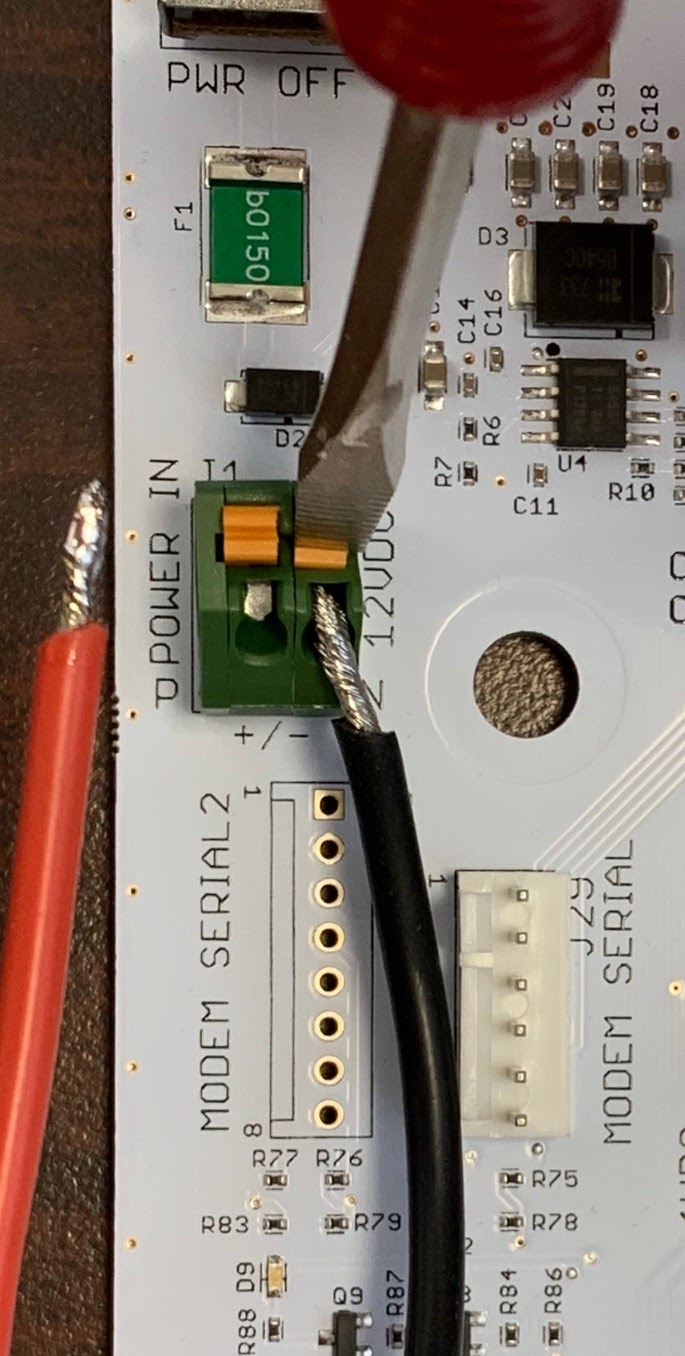
\includegraphics[width=0.25\textwidth,height=\textheight]{/Users/davidlapuma/Dropbox/CTT_Git/ctt_documentation/images/MODEM SERIAL2.jpg}
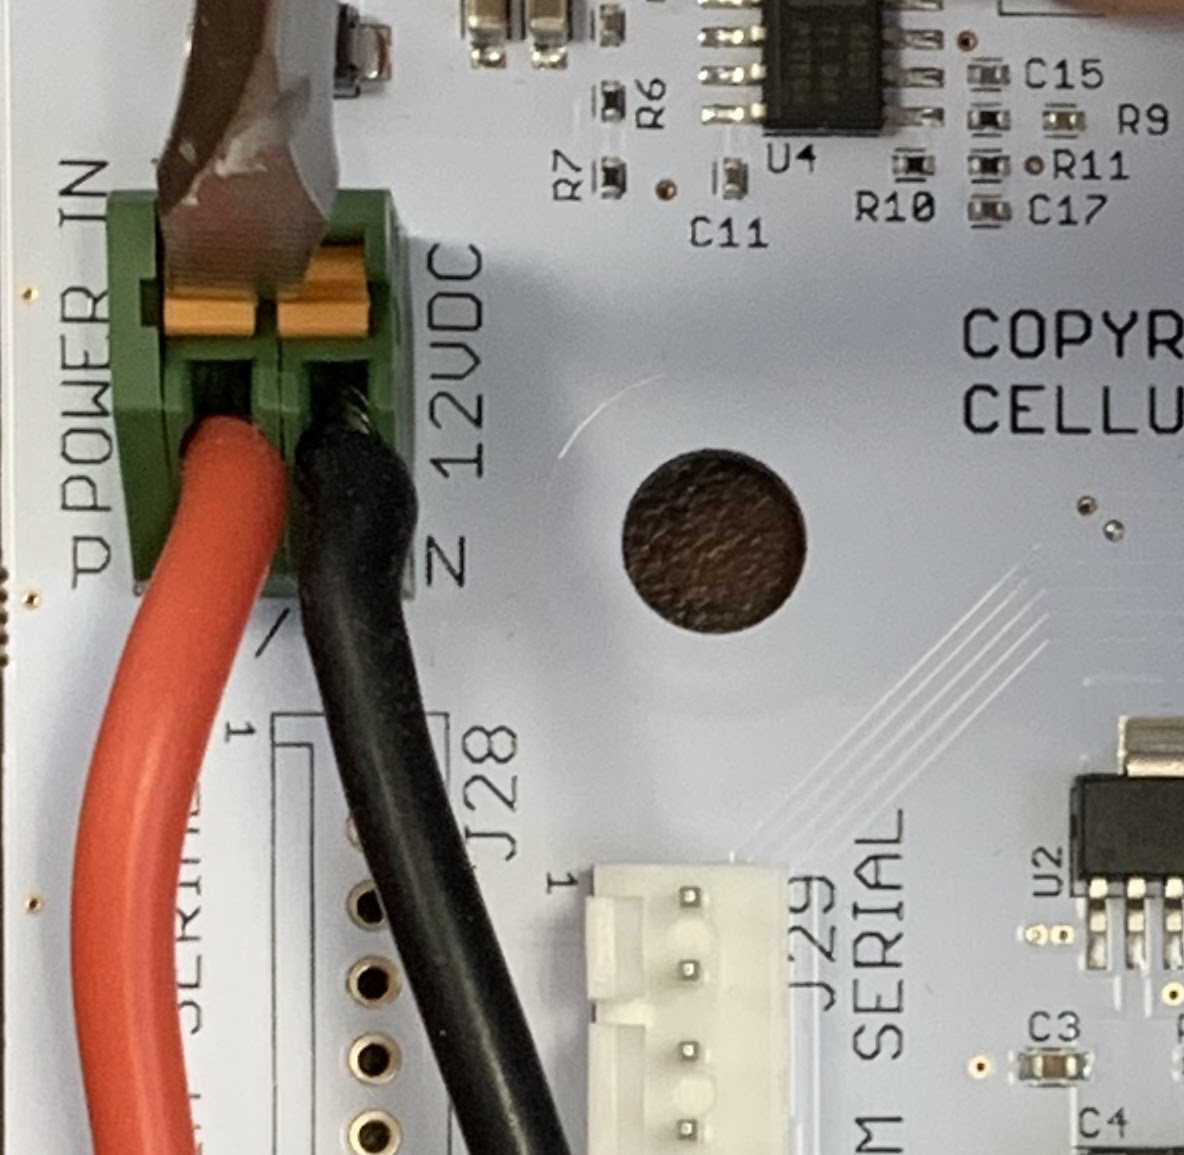
\includegraphics[width=0.25\textwidth,height=\textheight]{/Users/davidlapuma/Dropbox/CTT_Git/ctt_documentation/images/U POWER.jpg}

\hypertarget{initial-boot-up-of-a-sensorstation}{%
\subsection{Initial Boot-up of a
SensorStation}\label{initial-boot-up-of-a-sensorstation}}

\begin{enumerate}
\def\labelenumi{\arabic{enumi}.}
\tightlist
\item
  This is a simple set of instructions for the initial boot up of a
  SensorStation. Turn on the SensorStation using the slide switch on the
  left center of the SensorStation board.
\item
  The SensorStation board will show two constantly illuminated LEDs, an
  orange one and a green one on the left side of the board. There will
  also be green and blue flashing LEDs.
\end{enumerate}

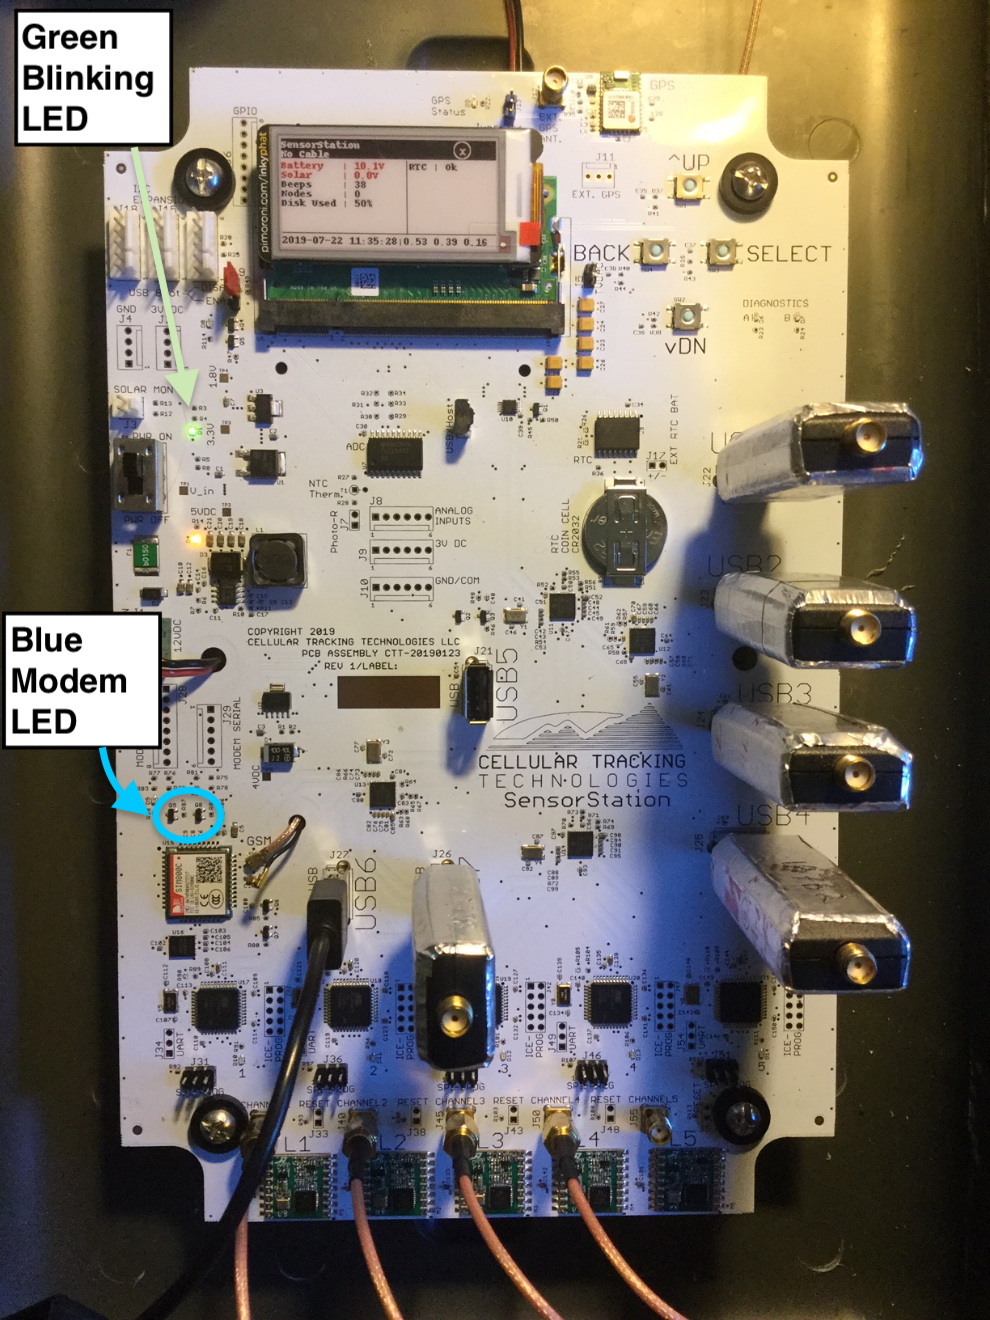
\includegraphics[width=0.4\textwidth,height=\textheight]{/Users/davidlapuma/Dropbox/CTT_Git/ctt_documentation/images/Battery.png}

\begin{enumerate}
\def\labelenumi{\arabic{enumi}.}
\setcounter{enumi}{2}
\tightlist
\item
  A normally operating SensorStation will present all four LEDs.
\item
  The Inkyphat display will show the CTT SensorStation welcome.
\end{enumerate}

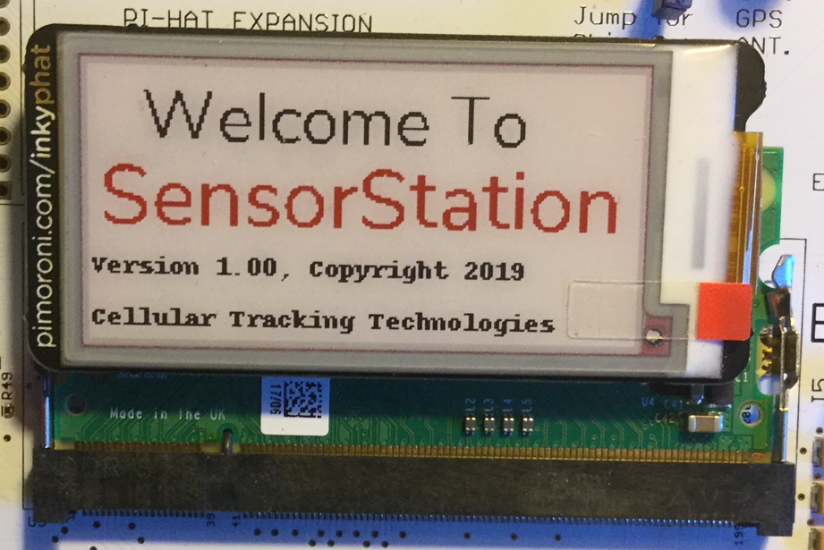
\includegraphics[width=0.5\textwidth,height=\textheight]{/Users/davidlapuma/Dropbox/CTT_Git/ctt_documentation/images/PI-HAT EXPANSION.png}

\begin{enumerate}
\def\labelenumi{\arabic{enumi}.}
\setcounter{enumi}{4}
\tightlist
\item
  The display normally updates every 90 seconds. During initial boot-up
  the display update usually takes longer than 90 seconds. Wait for the
  SensorStation to complete boot-up. Once the display updates it will
  change to the default operating screen display.
\end{enumerate}

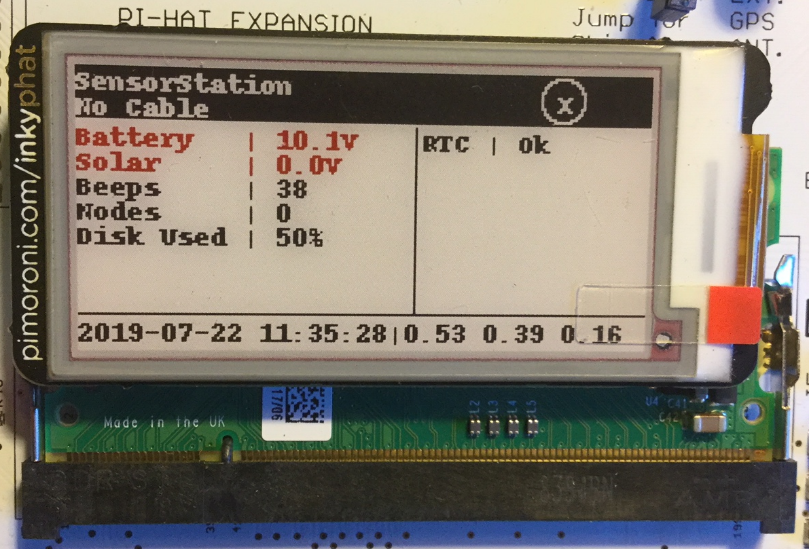
\includegraphics[width=0.5\textwidth,height=\textheight]{/Users/davidlapuma/Dropbox/CTT_Git/ctt_documentation/images/EXPANSION.png}

\begin{enumerate}
\def\labelenumi{\arabic{enumi}.}
\setcounter{enumi}{5}
\tightlist
\item
  This display shows that the SensorStation is operating, the battery
  voltage and the number of CTT transmitter detections (Beeps). Note
  that in the top bar the display shows ``No Cable''. This indicates
  that no Ethernet connection is available between the SensorStation
  board and a laptop computer.
\item
  Insert a USB to Ethernet connector into one of the open USB ports on
  the SensorStation.
\end{enumerate}

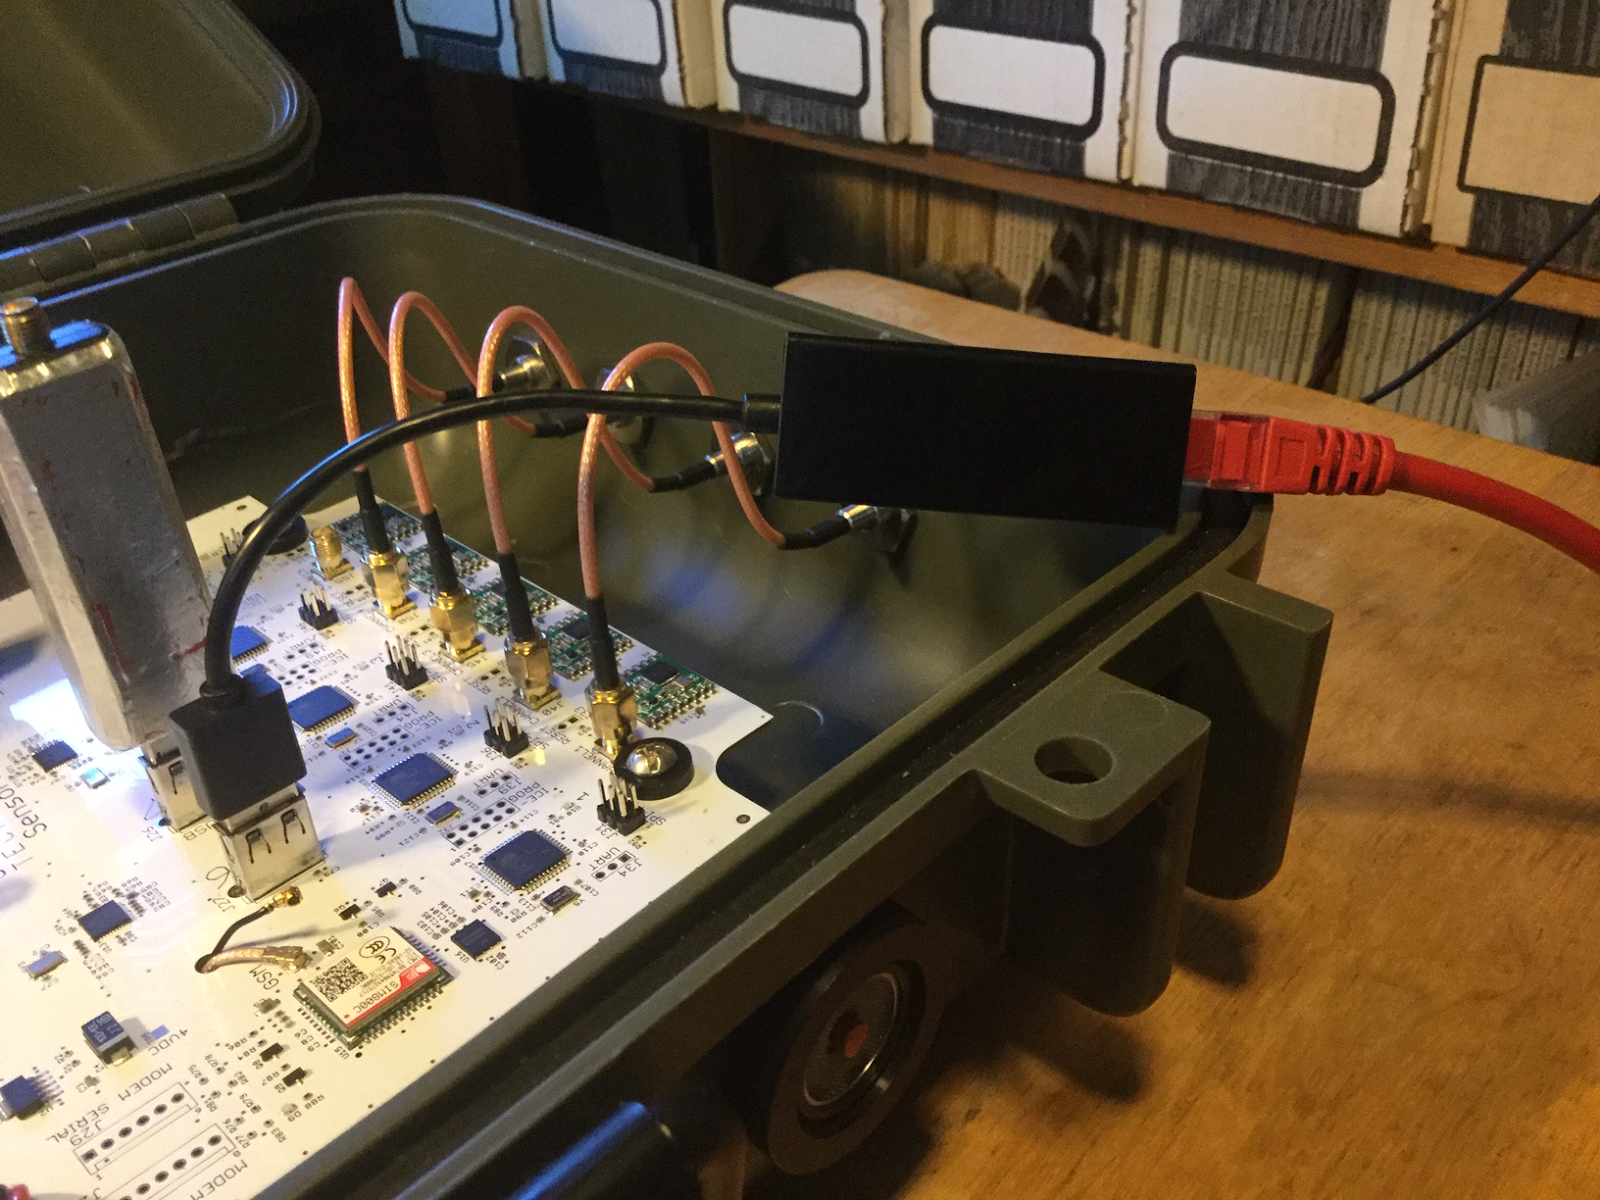
\includegraphics[width=0.5\textwidth,height=\textheight]{/Users/davidlapuma/Dropbox/CTT_Git/ctt_documentation/images/ethernetConnected.png}

\begin{enumerate}
\def\labelenumi{\arabic{enumi}.}
\setcounter{enumi}{7}
\tightlist
\item
  Connect your laptop to the SensorStation with an Ethernet cable. Wait
  for the Inkyphat display to update. Once the display updates you will
  see the IP address assigned to the combination of your laptop and
  SensorStation in the top bar of the display. In this example the
  assigned IP address is 169.254.54.185.
\end{enumerate}

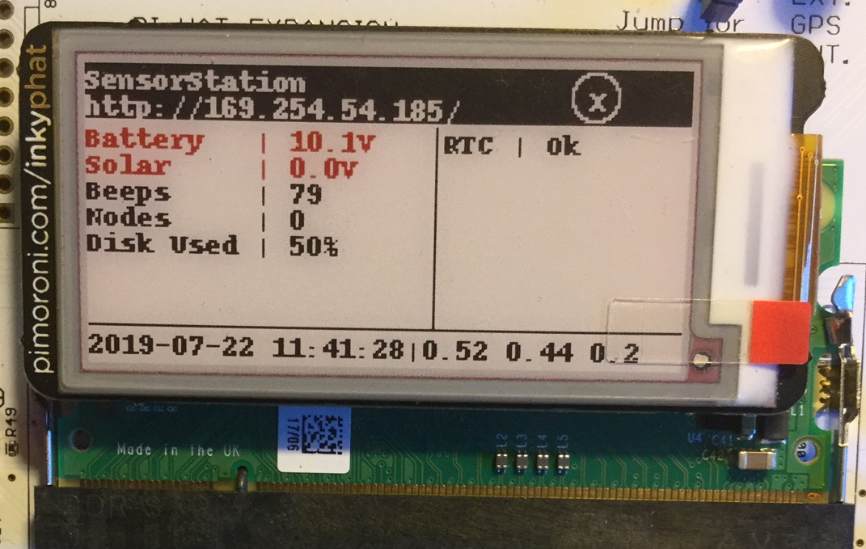
\includegraphics[width=0.5\textwidth,height=\textheight]{/Users/davidlapuma/Dropbox/CTT_Git/ctt_documentation/images/pimoroni.cominkyphat.jpg}

\begin{enumerate}
\def\labelenumi{\arabic{enumi}.}
\setcounter{enumi}{8}
\item
  Now you are ready to view the operating status of the SensorStation on
  two different, and necessary, web interfaces. There are separate web
  interfaces for the CTT and Motus (Sensorgnome) systems. Open your web
  browser and enter the IP address into the address bar to open a new
  web page. The CTT web interface will open.
\item
  If you have CTT LifeTags with you as test tags, they will show up as
  hits in the ``Tags'' window. The Station summary on the right includes
  information similar to the header of the familiar Sensorgnome display.
  The most important item is the ``ID'' number as that is needed to
  register the station with Motus. It also includes the time of the last
  boot and a boot counter. For more information on status scroll down
  through the display. The additional information includes windows for
  each of the five CTT antenna ports.
\item
  There is a section for data management that we can skip when setting
  up a station, that section may be more useful to us in the future.
  Just below data management there is a blue button ``Sensorgnome
  Interface''. Clicking on this button will open the familiar
  Sensorgnome web interface in a new window.
\end{enumerate}

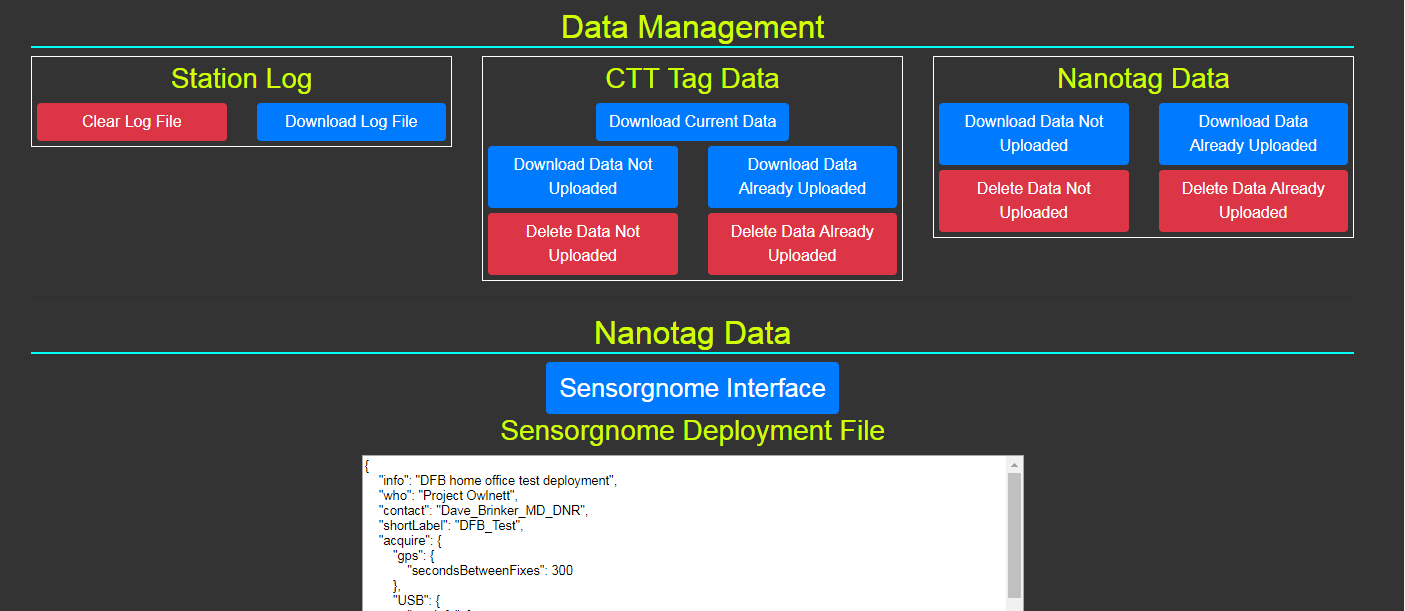
\includegraphics[width=0.75\textwidth,height=\textheight]{/Users/davidlapuma/Dropbox/CTT_Git/ctt_documentation/images/Data Management.png}

\begin{enumerate}
\def\labelenumi{\arabic{enumi}.}
\setcounter{enumi}{11}
\item
  FYI - you can edit the ``deployment.txt'' file in the provided box. At
  the bottom of the box there is a red ``Save Changes'' button. If you
  edit the deployment.txt file, do not forget to save your changes! The
  ``Reboot'' button also works as expected and pressing it will reboot
  the SensorStation.
\item
  You can leave both the CTT web interface and the Sensorgnome web
  interface open at the same time in your web browser and switch back
  and forth as necessary. The Sensorgnome web interface pretty much
  operates as expected. Please note that SensorStations do not use the
  GPS's clock to manage time and that you will always get the
  \textbf{\emph{PPS missing}} warning on the Sensorgnome interface.
\end{enumerate}

\begin{center}\rule{0.5\linewidth}{0.5pt}\end{center}

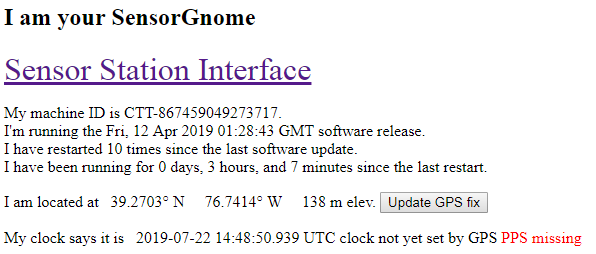
\includegraphics[width=0.75\textwidth,height=\textheight]{/Users/davidlapuma/Dropbox/CTT_Git/ctt_documentation/images/am your Sensor Gnome.png}

\begin{center}\rule{0.5\linewidth}{0.5pt}\end{center}

Clicking on ``Sensor Station Interface'' will open a new SensorStation
page and move you to it. It is generally easier to switch back and forth
between pages rather than clicking on the words to keep opening new
windows.

\begin{enumerate}
\def\labelenumi{\arabic{enumi}.}
\setcounter{enumi}{13}
\tightlist
\item
  You can set Funcube frequencies directly in the ``Devices'' window and
  most other functions should operate as expected. Currently there is no
  way to upload a tag database to the SensorStation.
\end{enumerate}

This should be enough to get us started and allow us to leave sites with
confidence that the SensorStations are operating correctly.

\begin{center}\rule{0.5\linewidth}{0.5pt}\end{center}

\hypertarget{appendix-iii-materials-list}{%
\section{Appendix III: Materials
List}\label{appendix-iii-materials-list}}

\begin{longtable}[]{@{}lllllll@{}}
\toprule
\begin{minipage}[b]{0.12\columnwidth}\raggedright
\textbf{Item}\strut
\end{minipage} & \begin{minipage}[b]{0.12\columnwidth}\raggedright
\textbf{Group}\strut
\end{minipage} & \begin{minipage}[b]{0.12\columnwidth}\raggedright
\textbf{Description}\strut
\end{minipage} & \begin{minipage}[b]{0.12\columnwidth}\raggedright
\textbf{Part Number}\strut
\end{minipage} & \begin{minipage}[b]{0.12\columnwidth}\raggedright
\textbf{Connection Type(s)}\strut
\end{minipage} & \begin{minipage}[b]{0.12\columnwidth}\raggedright
\textbf{Number Required}\strut
\end{minipage} & \begin{minipage}[b]{0.12\columnwidth}\raggedright
\textbf{Supplier Link}\strut
\end{minipage}\tabularnewline
\midrule
\endhead
\begin{minipage}[t]{0.12\columnwidth}\raggedright
A\strut
\end{minipage} & \begin{minipage}[t]{0.12\columnwidth}\raggedright
Comm.\strut
\end{minipage} & \begin{minipage}[t]{0.12\columnwidth}\raggedright
HO-432 Loop -- for receiving LifeTags omnidirectionally\strut
\end{minipage} & \begin{minipage}[t]{0.12\columnwidth}\raggedright
M2 HO-432\strut
\end{minipage} & \begin{minipage}[t]{0.12\columnwidth}\raggedright
Type N Female\strut
\end{minipage} & \begin{minipage}[t]{0.12\columnwidth}\raggedright
Depends on number of antennas\strut
\end{minipage} & \begin{minipage}[t]{0.12\columnwidth}\raggedright
\href{https://www.hamradio.com/detail.cfm?pid=H0-000720}{Link}\strut
\end{minipage}\tabularnewline
\begin{minipage}[t]{0.12\columnwidth}\raggedright
B\strut
\end{minipage} & \begin{minipage}[t]{0.12\columnwidth}\raggedright
Comm.\strut
\end{minipage} & \begin{minipage}[t]{0.12\columnwidth}\raggedright
A430S10 10 element yagi -- directional antenna for receiving distant
nodes and LifeTags\strut
\end{minipage} & \begin{minipage}[t]{0.12\columnwidth}\raggedright
Diamond Antenna A430S10\strut
\end{minipage} & \begin{minipage}[t]{0.12\columnwidth}\raggedright
SO-238 Female\strut
\end{minipage} & \begin{minipage}[t]{0.12\columnwidth}\raggedright
Depends on number of antennas\strut
\end{minipage} & \begin{minipage}[t]{0.12\columnwidth}\raggedright
\href{https://www.hamradio.com/detail.cfm?pid=H0-005816}{Link}\strut
\end{minipage}\tabularnewline
\begin{minipage}[t]{0.12\columnwidth}\raggedright
C\strut
\end{minipage} & \begin{minipage}[t]{0.12\columnwidth}\raggedright
Comm.\strut
\end{minipage} & \begin{minipage}[t]{0.12\columnwidth}\raggedright
433MHz 5dBi omni directional antenna -- for receiving nodes from any
direction, up to 700 meters away in some conditions\strut
\end{minipage} & \begin{minipage}[t]{0.12\columnwidth}\raggedright
Data Alliance A433O5\strut
\end{minipage} & \begin{minipage}[t]{0.12\columnwidth}\raggedright
Type N Male\strut
\end{minipage} & \begin{minipage}[t]{0.12\columnwidth}\raggedright
Depends on number of antennas\strut
\end{minipage} & \begin{minipage}[t]{0.12\columnwidth}\raggedright
\href{https://www.data-alliance.net/antenna-433mhz-5dbi-omnidirectional-fiberglass-w-n-male-vhf-uhf-marine/}{Link}\strut
\end{minipage}\tabularnewline
\begin{minipage}[t]{0.12\columnwidth}\raggedright
D\strut
\end{minipage} & \begin{minipage}[t]{0.12\columnwidth}\raggedright
Comm.\strut
\end{minipage} & \begin{minipage}[t]{0.12\columnwidth}\raggedright
Cable from Antenna to SensorStation\strut
\end{minipage} & \begin{minipage}[t]{0.12\columnwidth}\raggedright
USA Coax\strut
\end{minipage} & \begin{minipage}[t]{0.12\columnwidth}\raggedright
Depends on antenna and SensorStation type\strut
\end{minipage} & \begin{minipage}[t]{0.12\columnwidth}\raggedright
Depends on number of antennas\strut
\end{minipage} & \begin{minipage}[t]{0.12\columnwidth}\raggedright
\href{https://usacoax.com/cables.html}{Link}\strut
\end{minipage}\tabularnewline
\begin{minipage}[t]{0.12\columnwidth}\raggedright
E\strut
\end{minipage} & \begin{minipage}[t]{0.12\columnwidth}\raggedright
Mounting Hardware\strut
\end{minipage} & \begin{minipage}[t]{0.12\columnwidth}\raggedright
Tri-Pod\strut
\end{minipage} & \begin{minipage}[t]{0.12\columnwidth}\raggedright
Various, Amazon\strut
\end{minipage} & \begin{minipage}[t]{0.12\columnwidth}\raggedright
\strut
\end{minipage} & \begin{minipage}[t]{0.12\columnwidth}\raggedright
Depends on number of SensorStations\strut
\end{minipage} & \begin{minipage}[t]{0.12\columnwidth}\raggedright
\href{https://www.amazon.com/feet-Satellite-Tripod-Mount-2-Inch/dp/B0043OAI9M/ref=sr_1_3?keywords=antenna+tripod\&qid=1555017820\&s=electronics\&sr=1-3}{Link}\strut
\end{minipage}\tabularnewline
\begin{minipage}[t]{0.12\columnwidth}\raggedright
F\strut
\end{minipage} & \begin{minipage}[t]{0.12\columnwidth}\raggedright
Mounting Hardware\strut
\end{minipage} & \begin{minipage}[t]{0.12\columnwidth}\raggedright
Mast (electrical conduit)\strut
\end{minipage} & \begin{minipage}[t]{0.12\columnwidth}\raggedright
Lowes, Home Depot, Other Hardware Stores\strut
\end{minipage} & \begin{minipage}[t]{0.12\columnwidth}\raggedright
\strut
\end{minipage} & \begin{minipage}[t]{0.12\columnwidth}\raggedright
See Setup Guide\strut
\end{minipage} & \begin{minipage}[t]{0.12\columnwidth}\raggedright
\href{https://www.lowes.com/search?searchTerm=emt+conduit}{Link}\strut
\end{minipage}\tabularnewline
\begin{minipage}[t]{0.12\columnwidth}\raggedright
G\strut
\end{minipage} & \begin{minipage}[t]{0.12\columnwidth}\raggedright
AC Power\strut
\end{minipage} & \begin{minipage}[t]{0.12\columnwidth}\raggedright
110-250 A/C, 50Hz/60Hz, Universal power supply, USA adapter unless
specified\strut
\end{minipage} & \begin{minipage}[t]{0.12\columnwidth}\raggedright
Optional. If purchased separately its important to use 12V DC only\strut
\end{minipage} & \begin{minipage}[t]{0.12\columnwidth}\raggedright
\strut
\end{minipage} & \begin{minipage}[t]{0.12\columnwidth}\raggedright
\strut
\end{minipage} & \begin{minipage}[t]{0.12\columnwidth}\raggedright
\strut
\end{minipage}\tabularnewline
\begin{minipage}[t]{0.12\columnwidth}\raggedright
H\strut
\end{minipage} & \begin{minipage}[t]{0.12\columnwidth}\raggedright
Solar Power\strut
\end{minipage} & \begin{minipage}[t]{0.12\columnwidth}\raggedright
Panel 50 Watt\strut
\end{minipage} & \begin{minipage}[t]{0.12\columnwidth}\raggedright
Various\strut
\end{minipage} & \begin{minipage}[t]{0.12\columnwidth}\raggedright
50-100 Watt Panel is a good range. If you have the space 100W works
better under most conditions.\strut
\end{minipage} & \begin{minipage}[t]{0.12\columnwidth}\raggedright
one panel per station\strut
\end{minipage} & \begin{minipage}[t]{0.12\columnwidth}\raggedright
\href{https://www.amazon.com/Newpowa-Polycrystalline-Efficiency-Module-Marine/dp/B0725RZ22H/ref=sr_1_9?keywords=100\%2Bwatt\%2Bsolar\&qid=1552483408\&s=lawn-garden\&sr=1-9\&th=1}{Link}\strut
\end{minipage}\tabularnewline
\begin{minipage}[t]{0.12\columnwidth}\raggedright
I\strut
\end{minipage} & \begin{minipage}[t]{0.12\columnwidth}\raggedright
Solar Power\strut
\end{minipage} & \begin{minipage}[t]{0.12\columnwidth}\raggedright
12v Deep Cycle (Marine) Battery\strut
\end{minipage} & \begin{minipage}[t]{0.12\columnwidth}\raggedright
Everstart, others\strut
\end{minipage} & \begin{minipage}[t]{0.12\columnwidth}\raggedright
\strut
\end{minipage} & \begin{minipage}[t]{0.12\columnwidth}\raggedright
\strut
\end{minipage} & \begin{minipage}[t]{0.12\columnwidth}\raggedright
\href{https://www.walmart.com/ip/Everstart-Battery-Marine-12-Volt/868580543}{Link}\strut
\end{minipage}\tabularnewline
\begin{minipage}[t]{0.12\columnwidth}\raggedright
J\strut
\end{minipage} & \begin{minipage}[t]{0.12\columnwidth}\raggedright
Solar Power\strut
\end{minipage} & \begin{minipage}[t]{0.12\columnwidth}\raggedright
Charge Controller\strut
\end{minipage} & \begin{minipage}[t]{0.12\columnwidth}\raggedright
Various\strut
\end{minipage} & \begin{minipage}[t]{0.12\columnwidth}\raggedright
\strut
\end{minipage} & \begin{minipage}[t]{0.12\columnwidth}\raggedright
One per station\strut
\end{minipage} & \begin{minipage}[t]{0.12\columnwidth}\raggedright
\href{https://www.amazon.com/gp/product/B072MMDY4F?pf_rd_p=183f5289-9dc0-416f-942e-e8f213ef368b\&pf_rd_r=Z8QBVS0MGEQFA746ENSH}{Link}\strut
\end{minipage}\tabularnewline
\begin{minipage}[t]{0.12\columnwidth}\raggedright
K\strut
\end{minipage} & \begin{minipage}[t]{0.12\columnwidth}\raggedright
Solar Power\strut
\end{minipage} & \begin{minipage}[t]{0.12\columnwidth}\raggedright
Pole-mount for Solar\strut
\end{minipage} & \begin{minipage}[t]{0.12\columnwidth}\raggedright
\strut
\end{minipage} & \begin{minipage}[t]{0.12\columnwidth}\raggedright
Panel can be mounted on the ground but a tilt/pole mount makes it easier
to mount.\strut
\end{minipage} & \begin{minipage}[t]{0.12\columnwidth}\raggedright
1 set\strut
\end{minipage} & \begin{minipage}[t]{0.12\columnwidth}\raggedright
\href{https://www.amazon.com/WindyNation-Side-Solar-Panel-Mount/dp/B01NAKQMKW/ref=sr_1_4?keywords=solar+panel+pole+mount\&qid=1552483552\&s=lawn-garden\&sr=1-4}{Link}\strut
\end{minipage}\tabularnewline
\begin{minipage}[t]{0.12\columnwidth}\raggedright
L\strut
\end{minipage} & \begin{minipage}[t]{0.12\columnwidth}\raggedright
Node\strut
\end{minipage} & \begin{minipage}[t]{0.12\columnwidth}\raggedright
Mast\strut
\end{minipage} & \begin{minipage}[t]{0.12\columnwidth}\raggedright
Many\strut
\end{minipage} & \begin{minipage}[t]{0.12\columnwidth}\raggedright
The EMT for the SensorStation (2, 1.5, 1 1/4, 1 )\strut
\end{minipage} & \begin{minipage}[t]{0.12\columnwidth}\raggedright
\strut
\end{minipage} & \begin{minipage}[t]{0.12\columnwidth}\raggedright
\href{https://www.lowes.com/pd/Common-3-4-in-Actual-75-In-Metallic-Emt-10-ft-Conduit/3129553}{Link}\strut
\end{minipage}\tabularnewline
\begin{minipage}[t]{0.12\columnwidth}\raggedright
M\strut
\end{minipage} & \begin{minipage}[t]{0.12\columnwidth}\raggedright
Mounting Mast\strut
\end{minipage} & \begin{minipage}[t]{0.12\columnwidth}\raggedright
Clamp\strut
\end{minipage} & \begin{minipage}[t]{0.12\columnwidth}\raggedright
\strut
\end{minipage} & \begin{minipage}[t]{0.12\columnwidth}\raggedright
This should be the size of the bottom section of your mast- usually 1 ¼
to 2''\strut
\end{minipage} & \begin{minipage}[t]{0.12\columnwidth}\raggedright
\strut
\end{minipage} & \begin{minipage}[t]{0.12\columnwidth}\raggedright
\href{https://www.lowes.com/search?searchTerm=universal+strut+pipe+strap}{Link}\strut
\end{minipage}\tabularnewline
\begin{minipage}[t]{0.12\columnwidth}\raggedright
N\strut
\end{minipage} & \begin{minipage}[t]{0.12\columnwidth}\raggedright
Mounting Mast\strut
\end{minipage} & \begin{minipage}[t]{0.12\columnwidth}\raggedright
Mounting Rail\strut
\end{minipage} & \begin{minipage}[t]{0.12\columnwidth}\raggedright
Can be useful for mounting EMT mas on building or\strut
\end{minipage} & \begin{minipage}[t]{0.12\columnwidth}\raggedright
Two 2-3' sections\strut
\end{minipage} & \begin{minipage}[t]{0.12\columnwidth}\raggedright
\strut
\end{minipage} & \begin{minipage}[t]{0.12\columnwidth}\raggedright
\href{https://www.lowes.com/search?searchTerm=superstrut+gold-galvanized+half+slot+channel+strut}{Link}\strut
\end{minipage}\tabularnewline
\bottomrule
\end{longtable}

\end{document}
